% CVPR 2027 official author kit, tag CVPR2027-v1.
% Main document: pdfLaTeX + BibTeX. This project contains the confirmed Chapters 1--4.
\documentclass[10pt,twocolumn,letterpaper]{article}
\usepackage[review]{cvpr}
% Official teaser support. Main text fonts, margins, and line spacing are unchanged.
% Removed unused cuted: no strip environments are used.
\usepackage{caption}
\usepackage[T1]{fontenc}
\usepackage{microtype}


\raggedbottom
% Avoid stacking both single-column ablation tables above one column.
\setcounter{topnumber}{1}

\renewcommand{\paragraph}[1]{\par\addvspace{.5em}\noindent\textbf{#1}\hspace{.5em}\ignorespaces}
\usepackage{multicol}

\definecolor{cvprblue}{rgb}{0.21,0.49,0.74}
\usepackage[pagebackref,breaklinks,colorlinks,allcolors=cvprblue]{hyperref}
\def\confName{CVPR}
\def\confYear{2027}
\title{EfficientGeo: Distilling Foundation Models for Lightweight and Generalizable UAV-Based Cross-View Geo-Localization}
\author{Anonymous Authors}
\begin{document}
\maketitle
\begin{abstract}
UAV-based cross-view geo-localization requires accurate retrieval in unseen geographic regions under strict onboard computational constraints. Transferring visual foundation representations to a lightweight convolutional network involves both a substantial capacity gap and an architectural discrepancy. We present EfficientGeo, which uses a Transformer-based intermediate teacher and stage-specific supervision to transfer task-adapted foundation knowledge. To preserve discrimination among visually confusable locations across capacities, Teacher-Guided Hard Negative Distillation (TG-HND) matches positive-negative similarity margins on hard negatives selected by the foundation teacher in both retrieval directions. For cross-architecture transfer, Asymmetric Dual-Subspace Distillation (ADSD) constructs compact descriptor targets in a fixed PCA-based teacher subspace and an independently sampled random subspace. Student-side mappings learn these targets without full-dimensional feature alignment or intermediate-layer correspondence. Extensive experiments demonstrate that EfficientGeo achieves strong generalization performance in unseen geographic regions with fewer parameters and lower computational cost. Deployment on an NVIDIA Jetson Orin NX further confirms its practical efficiency for onboard inference.
\end{abstract}
\section{Introduction}
\label{sec:introduction}

UAV-based cross-view geo-localization (UAV-CVGL) aims to infer the geographic location corresponding to a UAV-view observation by retrieving geo-referenced satellite images.~\cite{zheng2020university}.
This task can provide visual localization support for UAV autonomous navigation, emergency rescue and infrastructure inspection in GNSS-denied environments.
Due to differences in imaging viewpoint, observation scale and visible scene content, the same location can exhibit significantly different appearances across views, while different locations may share similar building layouts and surface textures.
To this end, existing studies typically learn location-discriminative and view-robust representations via global and local feature alignment~\cite{wang2022lpn,dai2022fsra,deuser2023sample4geo}.
However, practical deployment of UAV-CVGL requires mounting an offline-trained model on a UAV and applying it to unseen geographic regions under limited onboard computation and strict inference latency constraints.
Therefore, developing a lightweight and generalizable model that enables accurate UAV-satellite retrieval in unseen geographic regions is essential for translating UAV-CVGL research into practice.

\begin{figure}[t]
\centering
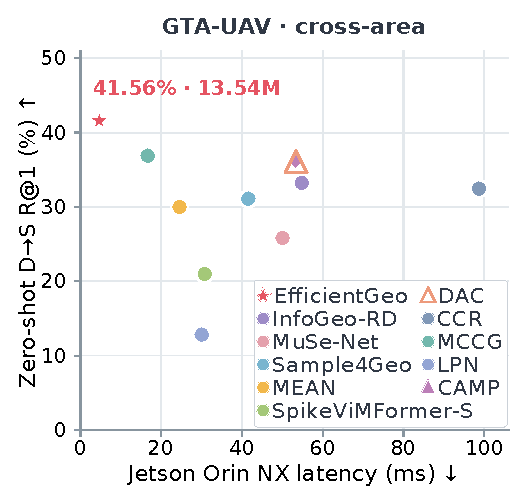
\includegraphics[width=\columnwidth]{EfficientGeo_GTA_CVPR_inside.pdf}


\caption{\textbf{Zero-shot retrieval accuracy versus query-encoding latency on Jetson Orin NX.} University-1652-trained models are evaluated on GTA-UAV cross-area.}
\label{fig:tradeoff}
\end{figure}

Motivated by this deployment requirement, some efforts have been made to pursue inference efficiency and reduce onboard cost through compact architectures, such as spike-driven transformer~\cite{chen2026spikevimformer} and ConvNeXt-Tiny backbones~\cite{chen2025mean}.
Another line of work targets cross-region generalization through object-centric structural alignment~\cite{zhang2026infogeo} and depth-aware geometric modeling~\cite{sun2026depthgeoloc}.
However, these two objectives are mutually constraining, since reducing model capacity may erode the representational richness that cross-region generalization depends on. This brings us to a fundamental question: how can we learn generalizable representations under strict model capacity constraints?

A promising direction is offered by self-supervised visual foundation models~\cite{caron2021dino,simeoni2025dinov3}, which encode general visual representations that transfer well across scenes and appearance variations. 
Such representations provide a strong prior for generalizable representation learning and help avoid overfitting to region-specific cues. 
However, task-agnostic foundation models are not aligned with the cross-view retrieval objective and even their compact variants can impose substantial computational demands for onboard inference.
Accordingly, this work focuses on transferring the generalization ability of a foundation model into a lightweight UAV-CVGL network for accurate UAV-satellite retrieval.

Knowledge distillation, which trains a compact student under the supervision of a stronger teacher, provides a natural route for such knowledge transfer~\cite{hinton2015distilling}. However, distilling a Transformer-based foundation model into a lightweight convolutional UAV-CVGL student is hindered by the substantial capacity gap and architectural discrepancy. 
Prior studies have shown that larger and stronger teachers do not guarantee better students~\cite{cho2019efficacy}, and that representation divergence across architectures further degrades feature-level distillation~\cite{liu2022crossarchitecture,hao2023ofa}.
Inspired by teacher assistant knowledge distillation~\cite{mirzadeh2020takd}, we insert a medium-scale, CVGL-specific Transformer as an intermediate teacher.
Architecturally homogeneous with the foundation teacher, it inherits the teacher's generalizable representations while specializing them for UAV-satellite retrieval. 
These intermediate descriptors are further turned into supervision targets tailored to the capacity and convolutional structure of the lightweight student, making the intermediate model a bridge between the foundation model and the compact student. 

In this paper, we propose EfficientGeo, a lightweight convolutional UAV-CVGL network trained through a two-stage distillation pipeline, in which a visual foundation model fine-tuned on the cross-view retrieval task serves as the teacher. 
In the first stage, we introduce Teacher-Guided Hard Negative Distillation (TG-HND), where the teacher identifies hard negatives and guides a Transformer-based intermediate model to mimic the corresponding positive-negative similarity margins.
Complementing this ranking guidance, multi-level feature calibration aligns the intermediate model’s hidden representations with fused features from multiple teacher layers, encouraging more discriminative feature learning.
In the second stage, Asymmetric Dual-Subspace Distillation (ADSD) projects the intermediate descriptor into a deterministic dominant subspace that carries its principal directions and an independently sampled random subspace that contributes complementary constraints, yielding low-dimensional supervision targets. Supervising these low-dimensional coordinates relieves the student from reproducing representational directions beyond its capacity, making cross-architecture supervision well-posed and helping to preserve the generalizable representations inherited in the first stage.

 Both stages further adopt distillation-guided Sharpness-Aware Minimization (SAM)~\cite{foret2021sam}  as an optimizer-level regularizer, which seeks flat minima for the distilled objectives and improves robustness. Through this pipeline, the lightweight EfficientGeo retains much of the generalization capability of the foundation model while remaining compact for onboard retrieval, achieving both efficient inference and generalizable cross-view geo-localization.

Our main contributions are summarized as follows:
\begin{itemize}
  \item We establish a two-stage cross-architecture distillation framework for UAV-CVGL that distill a fine-tuned visual foundation model to a lightweight convolutional student through a Transformer-based intermediate model, yielding EfficientGeo as a lightweight and generalizable solution for onboard cross-view geo-localization.
  \item We introduce ADSD for cross-architecture transfer. It projects each teacher descriptor onto principal directions and independently sampled random directions, then trains a separate student mapping for each fixed set of directions.
  \item Trained on University-1652, the reparameterized 13.54\,M-parameter student achieves zero-shot drone-to-satellite R@1 of 94.35\% on SUES-200, averaged over four flight heights, and 41.56\% on GTA-UAV cross-area. The same encoder encodes a query image in 4.65\,ms on Jetson Orin NX.

\end{itemize}


\section{Related Work}
\label{sec:related_work}

\subsection{UAV-based Cross-View Geo-Localization}

UAV-based retrieval requires discriminative representations despite large changes in viewpoint, scale, and appearance. LPN~\cite{wang2022lpn} uses square-ring partitions to capture local patterns and surrounding context, while FSRA~\cite{dai2022fsra} aligns regions obtained from Transformer features across views. Sample4Geo~\cite{deuser2023sample4geo} improves representation learning through symmetric contrastive learning and hard negative sampling.

Generalization to unseen geographic regions is another important consideration. DAC~\cite{xia2024dac} combines cross-view feature alignment with scene consistency, and InfoGeo~\cite{zhang2026infogeo} aligns object-centric structural relations while suppressing view-specific information. Pretrained visual models also provide transferable representations for retrieval. In the related task of visual place recognition, AnyLoc~\cite{keetha2023anyloc} aggregates self-supervised features, while SALAD~\cite{izquierdo2024salad} fine-tunes DINOv2 and aggregates local features through optimal transport. These studies motivate the use of pretrained visual representations in UAV-satellite retrieval.

For efficient deployment, MEAN~\cite{chen2025mean} uses a lightweight backbone with multi-level feature enhancement and cross-view alignment, while SpikeViMFormer~\cite{chen2026spikevimformer} adopts a spike-driven Transformer backbone. Knowledge distillation provides another route to compact models. DepthGeoLoc~\cite{sun2026depthgeoloc} transfers depth-aware structural knowledge through coarse-to-fine distillation. MobileGeo~\cite{sun2025mobilegeo} uses hierarchical distillation and uncertainty-aware prediction alignment, together with view selection at inference. EfficientGeo also uses distillation to train a lightweight model, aiming for accurate retrieval in unseen geographic regions under onboard computational constraints.

\subsection{Knowledge Distillation}

A large capacity gap can make it difficult for a compact student to learn directly from a stronger teacher~\cite{cho2019efficacy}. Teacher assistant distillation~\cite{mirzadeh2020takd} introduces an intermediate-sized model to bridge this gap, while densely guided knowledge distillation~\cite{son2021dgkd} extends this strategy to multiple assistants. Inspired by these studies, EfficientGeo uses a Transformer-based intermediate teacher to transfer task-adapted foundation knowledge to a lightweight convolutional student.

Knowledge can also be transferred through relationships among samples. DarkRank~\cite{chen2018darkrank} and RKD~\cite{park2019rkd} distill similarity-based rankings and geometric relationships, respectively. For retrieval, Margin-MSE~\cite{hofstatter2020marginmse} matches score differences between relevant and non-relevant passages. GeoMFD~\cite{chen2026geomfd} transfers positive-negative similarity margins on teacher-selected hard negatives in both retrieval directions to reduce forgetting during continual adaptation. In our setting, the task-adapted foundation teacher transfers positive-negative similarity margins to a smaller intermediate teacher, using hard negatives selected by the foundation teacher.

Transferring features across different architectures is also challenging because Transformer and convolutional models represent visual information differently. Existing methods use projection modules~\cite{liu2022crossarchitecture,hao2023ofa} or combine heterogeneous teacher and student modules~\cite{li2025fbt} to facilitate transfer. VkD~\cite{miles2024vkd} aligns teacher and student features using an orthogonal projection and task-specific normalization. In EfficientGeo, the convolutional student learns compact descriptor targets obtained from two fixed projections of the intermediate teacher. The teacher subspace captures principal directions of its representations, while an independently sampled random subspace provides a second target. This design does not require correspondence between intermediate layers of the Transformer teacher and the convolutional student.

\section{Method}
\label{sec:method}
\subsection{Problem Formulation and Overview}
\label{sec:overview}

Each training batch contains $N$ UAV--satellite image pairs
$\{(x_i^u,x_i^s)\}_{i=1}^{N}$ from distinct locations,
where $x_i^u$ and $x_i^s$ depict the same location.

Let $\mathcal{T}$, $\mathcal{M}$, and $\mathcal{S}$ denote
the task-adapted foundation teacher, the intermediate
teacher, and the student, respectively. Within each model,
the two views share an encoder that produces an
$\ell_2$-normalized descriptor $z(x)$. We use model
subscripts when distinguishing descriptors or similarities
from different models.

As shown in Fig.~\ref{fig:framework}, EfficientGeo adopts
a two-stage distillation framework. In Stage~I, the frozen
$\mathcal{T}$ (DINOv3 ViT-7B) supervises $\mathcal{M}$
(DINOv3 ViT-B) through TG-HND and multi-level feature
calibration. In Stage~II, the frozen $\mathcal{M}$
supervises $\mathcal{S}$ (RepViT-M1.5) through ADSD.
Both stages are optimized with DG-SAM.

\begin{figure*}[t]
\centering
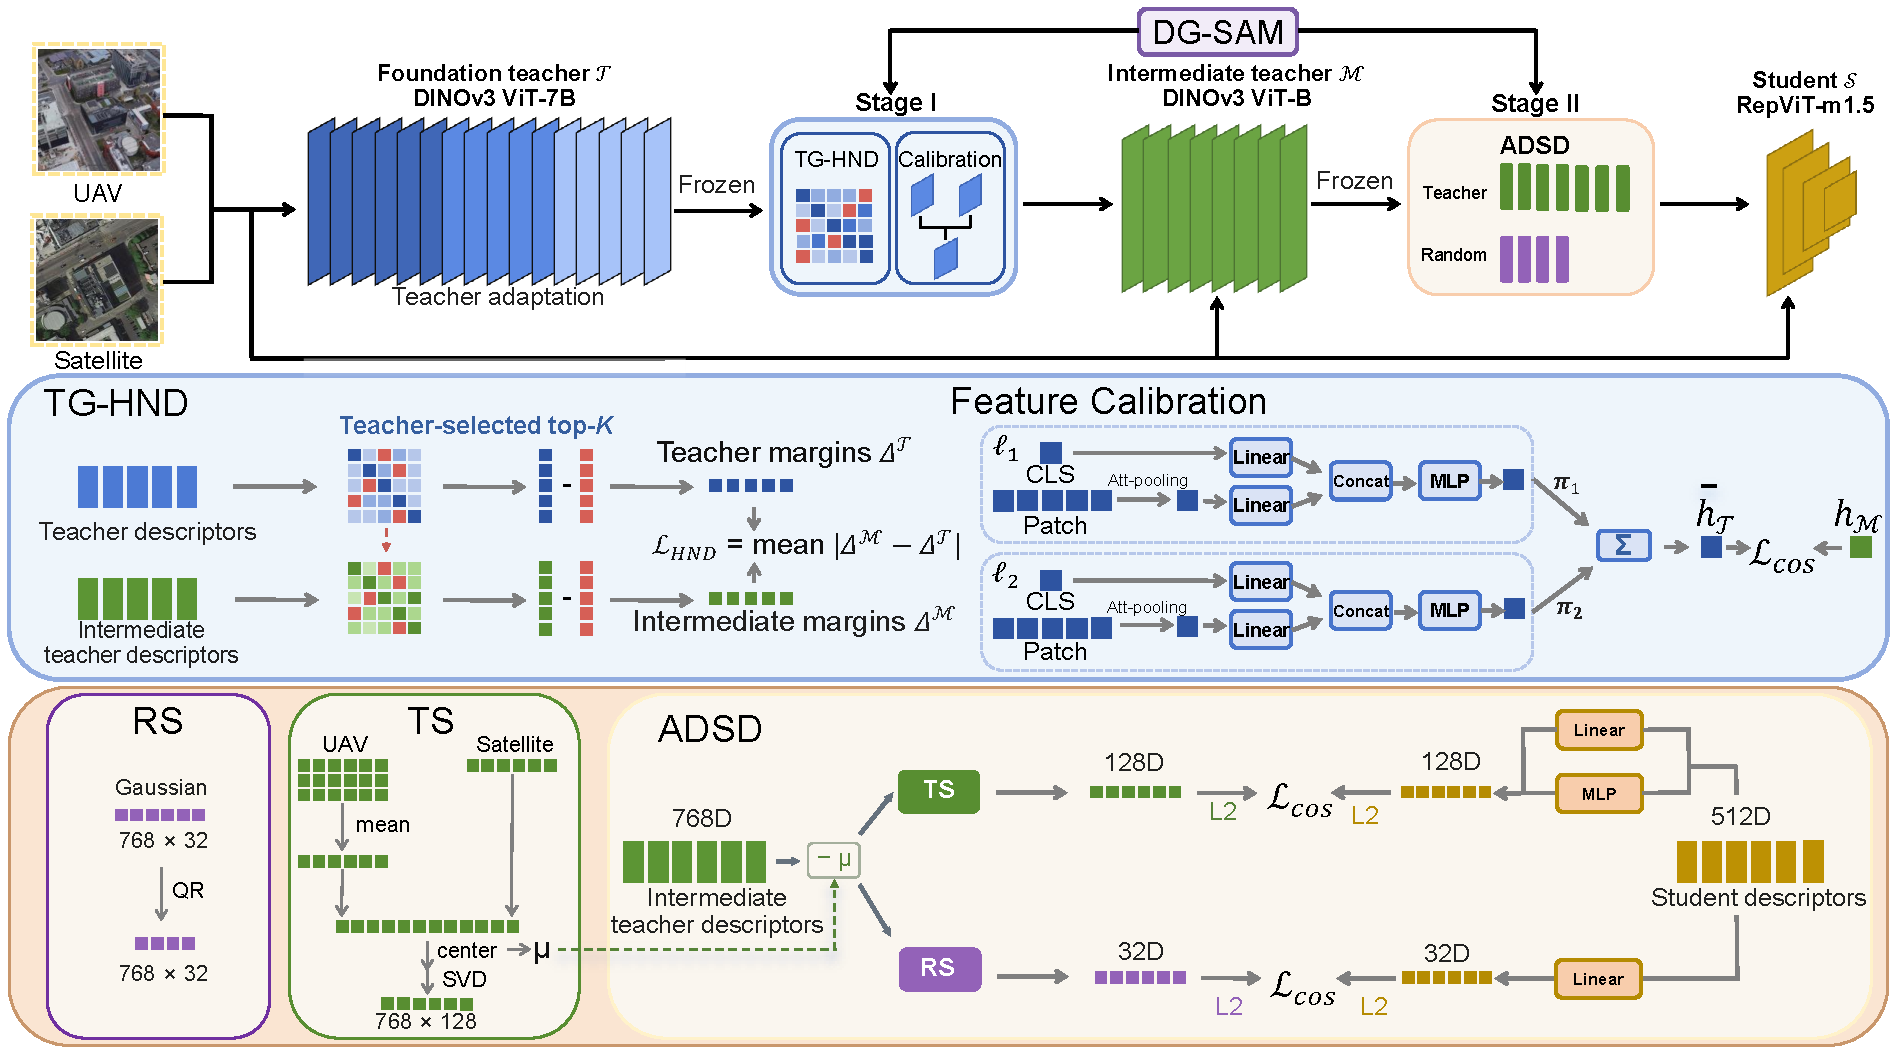
\includegraphics[width=0.96\textwidth]{figure2-128-32.pdf}
\caption{Overview of EfficientGeo. Stage~I uses TG-HND and auxiliary feature calibration for cross-capacity transfer. Stage~II uses ADSD for cross-architecture transfer through the PCA-based Teacher Subspace (TS) and an independently sampled Random Subspace (RS).}
\label{fig:framework}
\end{figure*}


\paragraph{Retrieval objective.}
For the encoder being trained, let
$C\in\mathbb{R}^{N\times N}$ be its UAV-to-satellite
similarity matrix, where
$C_{ij}=z(x_i^u)^\top z(x_j^s)$. The diagonal entry
$C_{ii}$ corresponds to a positive pair, while
$C_{ij}$ with $j\ne i$ corresponds to a negative pair.

For the two retrieval directions
$\omega\in\{u\rightarrow s,s\rightarrow u\}$, we use
$C^{u\rightarrow s}=C$ and
$C^{s\rightarrow u}=C^\top$. Thus, $C_{ij}^{\omega}$
is the similarity between query $i$ and candidate $j$
in direction $\omega$.

Let $\tau>0$ be a learnable temperature and
$q_{ij}=(1-\eta)\mathbf{1}[i=j]+\eta/N$ be the target
probability, where $\eta$ is the label-smoothing factor.
The bidirectional InfoNCE loss~\cite{deuser2023sample4geo}
is
\begin{equation}
\mathcal{L}_{\mathrm{ret}}
=-\frac{1}{2N}
\sum_{\omega}\sum_{i,j=1}^{N}
q_{ij}
\log
\frac{\exp(C_{ij}^{\omega}/\tau)}
{\sum_{k=1}^{N}\exp(C_{ik}^{\omega}/\tau)}.
\label{eq:retrieval}
\end{equation}
We use this loss to adapt $\mathcal{T}$ and to train
$\mathcal{M}$ and $\mathcal{S}$ in Stages~I and~II,
respectively. When needed, a superscript on
$\mathcal{L}_{\mathrm{ret}}$ identifies the corresponding
model. Each model has its own temperature. We set
$\eta=0$ for $\mathcal{T}$ and $\mathcal{M}$, and
$\eta=0.1$ for $\mathcal{S}$.

\paragraph{Teacher adaptation.}
Before distillation, we adapt pretrained DINOv3 ViT-7B
using $\mathcal{L}_{\mathrm{ret}}^{\mathcal{T}}$.
We freeze its early Transformer blocks, apply
LoRA~\cite{hu2022lora} to intermediate blocks, and
fully fine-tune the final blocks. Further implementation details are provided in Section A.1 of the supplementary material.

\subsection{Teacher-Guided Hard Negative Distillation}
\label{sec:tghnd}

\paragraph{Teacher-guided margin transfer.}
For query $i$ and retrieval direction $\omega$, let
$C_{\mathcal{T}}^\omega$ and
$C_{\mathcal{M}}^\omega$ be the similarity matrices of
$\mathcal{T}$ and $\mathcal{M}$, respectively. The teacher
selects the indices $\mathcal{H}_i^\omega$ of its $K=5$
highest-scoring in-batch negatives. The positive--negative
margin measures the similarity gap between the positive
candidate $i$ and a selected negative candidate $j$:
\begin{equation}
\mathcal{H}_i^\omega
=\operatorname{TopK}_{j\ne i}
C_{\mathcal{T},ij}^\omega,
\qquad
\Delta_{ij}^\omega
=C_{ii}^\omega-C_{ij}^\omega.
\label{eq:hnd_candidates_margins}
\end{equation}
We write $\Delta_{\mathcal{T},ij}^\omega$ and
$\Delta_{\mathcal{M},ij}^\omega$ for the margins computed
by the teacher and intermediate model, respectively.
We align these margins on the selected negatives:
\begin{equation}
\mathcal{L}_{\mathrm{HND}}
=\frac{1}{2NK}
\sum_{\omega}
\sum_{1\leq i\leq N}
\sum_{j\in\mathcal{H}_i^\omega}
\left|
\Delta_{\mathcal{M},ij}^\omega
-\Delta_{\mathcal{T},ij}^\omega
\right|.
\label{eq:hnd_loss}
\end{equation}

\paragraph{Auxiliary multi-level feature calibration.}
To complement margin transfer, we extract the
classification (CLS) token and patch tokens from two
selected layers of $\mathcal{T}$ for each image $x$.
At each layer, attention pooling summarizes the patch
tokens, and a layer-specific bridge combines the pooled
feature with the CLS token and maps it to the
hidden-feature dimension of $\mathcal{M}$. Let
$\mathbf{h}_{\mathcal{T}}^{(1)}(x)$ and
$\mathbf{h}_{\mathcal{T}}^{(2)}(x)$ be the resulting
features. The fused teacher target is
\[
\bar{\mathbf{h}}_{\mathcal{T}}(x)
=\pi_1\mathbf{h}_{\mathcal{T}}^{(1)}(x)
+\pi_2\mathbf{h}_{\mathcal{T}}^{(2)}(x),
\]
where $\pi_1$ and $\pi_2$ are learned, softmax-normalized
weights shared across images and views.

Let $\mathbf{h}_{\mathcal{M}}(x)$ be the CLS feature from
a selected hidden layer of $\mathcal{M}$. For
$i=1,\ldots,N$ and $v\in\{u,s\}$, we align it with
the fused teacher target using a cosine loss:
\begin{equation}
\mathcal{L}_{\mathrm{cal}}
=\frac{1}{2N}\sum_{i,v}
\left[
1-\cos\left(
\mathbf{h}_{\mathcal{M}}(x_i^v),
\bar{\mathbf{h}}_{\mathcal{T}}(x_i^v)
\right)
\right].
\label{eq:calibration_loss}
\end{equation}
The calibration modules are trained jointly with $\mathcal{M}$.
Bridge details are provided in Section A.3 of the supplementary material.

The Stage~I objective is
\begin{equation}
\mathcal{L}_{\mathrm{I}}
=\mathcal{L}_{\mathrm{ret}}^{\mathcal{M}}
+\lambda_{\mathrm{HND}}\mathcal{L}_{\mathrm{HND}}
+\lambda_{\mathrm{cal}}\mathcal{L}_{\mathrm{cal}}.
\label{eq:stage_one_objective}
\end{equation}


\subsection{Asymmetric Dual-Subspace Distillation}
\label{sec:adsd}
\paragraph{Dual-subspace target construction.}
To supervise $\mathcal{S}$, we project the descriptors of
$\mathcal{M}$ onto a Teacher Subspace (TS) and a Random
Subspace (RS). For each training location, the UAV centroid is obtained
by averaging the descriptors of its unaugmented UAV images
and $\ell_2$-normalizing the result, while the satellite
centroid is the descriptor of its single unaugmented
satellite image. Let $\mu$ be the mean of
these centroids.
We apply principal component analysis (PCA) to the
centered centroids and use the leading directions as the
TS basis $P$. Independently, we orthonormalize Gaussian
vectors to obtain the RS basis $R$. The two bases are not
constrained to be mutually orthogonal. Both bases and
$\mu$ remain fixed during student training. 
Further details of the centroid and subspace construction
are provided in the supplementary material.

For an augmented image $x$, $\mathcal{M}$ produces the
descriptor $z_{\mathcal{M}}(x)$. The two targets for
$\mathcal{S}$ are
\begin{equation}
\begin{aligned}
t_p(x)&=\operatorname{norm}\!\left(
P^\top[z_{\mathcal{M}}(x)-\mu]\right),\\
t_r(x)&=\operatorname{norm}\!\left(
R^\top[z_{\mathcal{M}}(x)-\mu]\right),
\end{aligned}
\label{eq:adsd_targets}
\end{equation}
where $\operatorname{norm}(\cdot)$ denotes
$\ell_2$ normalization.

\paragraph{Asymmetric student mappings.}
For the same image $x$, $\mathcal{S}$ produces the
descriptor $z_{\mathcal{S}}(x)$. The student predictions
corresponding to TS and RS are
\begin{equation}
\begin{aligned}
\hat{t}_p(x)&=\operatorname{norm}\!\left(
W_pz_{\mathcal{S}}(x)+b_p
+\gamma f(z_{\mathcal{S}}(x))\right),\\
\hat{t}_r(x)&=\operatorname{norm}\!\left(
W_rz_{\mathcal{S}}(x)+b_r\right),
\end{aligned}
\label{eq:adsd_student_heads}
\end{equation}
where $W_p,W_r$ and $b_p,b_r$ are the weights and biases
of the linear mappings, $f$ is a learnable two-layer
multilayer perceptron (MLP) with Gaussian error linear
unit (GELU) activation, and $\gamma$ is a learnable scalar.
Both mappings are shared across views, with initialization
details provided in the supplementary material.

For $k\in\{p,r\}$, $i=1,\ldots,N$, and $v\in\{u,s\}$,
we align each student prediction with its corresponding
teacher target using a cosine loss:
\begin{equation}
\mathcal{L}_k
=\frac{1}{2N}\sum_{i,v}
\left[
1-\cos\left(\hat{t}_k(x_i^v),t_k(x_i^v)\right)
\right].
\label{eq:adsd_branch_loss}
\end{equation}

\paragraph{Branch weighting.}
Gradient-balanced weighting (GBW) uses a separately
optimized gate to adjust the branch weights $w_p$ and
$w_r$, encouraging the weighted gradient norms of the
two losses with respect to the shared student descriptor
to be similar. Further details of the gate objective and
gradient computation are provided in Section A.4 of the supplementary
material.

The Stage~II objective is
\begin{equation}
\mathcal{L}_{\mathrm{II}}
=\mathcal{L}_{\mathrm{ret}}^{\mathcal{S}}
+\lambda_{\mathrm{ADSD}}\!\left(
w_p\mathcal{L}_p+w_r\mathcal{L}_r
\right).
\label{eq:stage_two_objective}
\end{equation}
The distillation weight $\lambda_{\mathrm{ADSD}}$ increases
from $0.04$ to $0.2$ in steps of $0.04$ over the first five
epochs and remains fixed thereafter.

\subsection{Optimization and Inference}
\label{sec:optimization}

\paragraph{Distillation-guided optimization.}
To encourage more stable knowledge transfer under parameter
perturbations, we apply distillation-guided sharpness-aware
minimization (DG-SAM) in both stages, based on
SAM~\cite{foret2021sam}. DG-SAM constructs the perturbation
using only the distillation terms in each stage objective.

Let $g_{\mathrm{KD}}$ denote the gradient of the weighted
distillation terms in the current stage objective: TG-HND
and feature calibration in Stage~I
(Eq.~\eqref{eq:stage_one_objective}), and ADSD in Stage~II
(Eq.~\eqref{eq:stage_two_objective}). The gradient is taken
with respect to the trainable parameters $\phi$ of the
recipient model and its auxiliary modules. The resulting
perturbation is
\begin{equation}
\varepsilon_{\phi}
=\rho\frac{g_{\mathrm{KD}}}
{\|g_{\mathrm{KD}}\|_2+\delta},
\label{eq:dgsam_perturbation}
\end{equation}
where $\rho=0.1$ controls the perturbation magnitude and
$\delta=10^{-12}$ ensures numerical stability.

On the same batch, we compute the gradient of the complete
stage objective, including both retrieval and distillation,
at $\phi+\varepsilon_{\phi}$, treating the perturbation as
fixed. We then restore $\phi$ and update it using this
gradient. The separately optimized GBW gate in Stage~II is
excluded from the perturbation. Further details of the
DG-SAM update are provided in Section A.5 of the supplementary material.

\paragraph{Inference.}
At inference, the student $\mathcal{S}$ uses the same
RepViT-M1.5 encoder~\cite{wang2024repvit} for both UAV
and satellite images, producing 512-dimensional descriptors.
Gallery images are ranked by cosine similarity between their
descriptors and the query descriptor. For deployment, RepViT's
native structural reparameterization can be applied while
retaining the post-pooling batch normalization.

\section{Experiments}
\label{sec:experiments}
\begin{table*}[t]
\centering
\caption{University-1652 retrieval performance (\%) and model efficiency. FPS is measured on Jetson Orin NX.}
\label{tab:university}
\footnotesize
\setlength{\tabcolsep}{3pt}
\begin{tabular*}{\textwidth}{@{\extracolsep{\fill}}lcrrrrrrrr@{}}
\toprule
\raisebox{-4.5pt}[0pt][0pt]{Method} & \raisebox{-4.5pt}[0pt][0pt]{Venue / Year} & \raisebox{-4.5pt}[0pt][0pt]{Input} & \raisebox{-4.5pt}[0pt][0pt]{Params (M)$\downarrow$} & \raisebox{-4.5pt}[0pt][0pt]{FLOPs (G)$\downarrow$} & \raisebox{-4.5pt}[0pt][0pt]{FPS$\uparrow$} & \multicolumn{2}{c}{D$\rightarrow$S} & \multicolumn{2}{c}{S$\rightarrow$D} \\
 & & & & & & R@1$\uparrow$ & AP$\uparrow$ & R@1$\uparrow$ & AP$\uparrow$ \\
\midrule
LPN~\cite{wang2022lpn}$^{r}$ & TCSVT 2022 & 256 & 27.71 & 16.28 & 33.28 & 75.77 & 79.09 & 88.02 & 76.01 \\
MuSe-Net~\cite{wang2024musenet}$^{r}$ & PR 2024 & 256 & 26.60 & 25.88 & 19.98 & 74.73 & 78.09 & 87.87 & 75.52 \\
Sample4Geo~\cite{deuser2023sample4geo}$^{r}$ & ICCV 2023 & 384 & 87.57 & 90.83 & 24.06 & 92.66 & 93.81 & 95.15 & 91.39 \\
MEAN~\cite{chen2025mean} & TGRS 2025 & 384 & 27.82 & 26.46 & 40.74 & 93.55 & 94.53 & 96.01 & 92.08 \\
CAMP~\cite{wu2024camp}$^{r}$ & TGRS 2024 & 384 & 87.71 & 90.83 & 18.73 & 94.42 & 95.35 & 96.15 & 92.72 \\
DAC~\cite{xia2024dac}$^{r}$ & TCSVT 2024 & 384 & 87.57 & 90.83 & 18.76 & \textbf{94.68} & \textbf{95.51} & \textbf{96.43} & \textbf{93.80} \\
CCR~\cite{du2024ccr}$^{r}$ & TCSVT 2024 & 384 & 121.68 & 90.96 & 10.13 & 92.95 & 94.16 & 95.72 & 92.55 \\
MCCG~\cite{shen2024mccg}$^{r}$ & TCSVT 2024 & 256 & 29.00 & 11.77 & 60.05 & 89.59 & 91.33 & 94.44 & 89.62 \\
SpikeViMFormer-S~\cite{chen2026spikevimformer}$^{r}$ & TCSVT 2026 & 384 & 18.63 & 50.12 & 32.49 & 88.00 & 89.96 & 92.30 & 87.11 \\
InfoGeo-RD~\cite{zhang2026infogeo}$^{r}$ & ICML 2026 & 448 & 91.57 & 223.50 & 18.24 & 89.82 & 91.43 & 95.29 & 90.32 \\
DepthGeoLoc~\cite{sun2026depthgeoloc} & TGRS 2026 & 252 & 28.57 & 11.63 & -- & 92.75 & 93.82 & 94.58 & 91.56 \\
MobileGeo~\cite{sun2025mobilegeo} & arXiv 2025 & 224 & 28.57 & \textbf{4.45} & -- & 93.87 & 94.83 & 95.72 & 92.57 \\
\midrule
\textbf{EfficientGeo} & Ours & 256 & 13.62 & 6.07 & 137.67 & 93.20 & 94.28 & 95.15 & 92.34 \\
\textbf{EfficientGeo + Rep.} & Ours & 256 & \textbf{13.54} & 6.01 & \textbf{214.34} & 93.14 & 94.23 & 95.29 & 92.32 \\
\bottomrule
\end{tabular*}
\par\smallskip{\footnotesize\raggedright $^{r}$: reproduced results. Other results are paper-reported. DepthGeoLoc: student. MobileGeo: without MSRM. Rep.: reparameterized. --: unavailable.\par}
\end{table*}



\subsection{Experimental Setup}
\label{sec:experimental_setup}

\paragraph{Datasets.}
To assess the cross-dataset generalization of EfficientGeo,
we train the model on University-1652~\cite{zheng2020university}
and evaluate it on SUES-200~\cite{zhu2023sues} and
GTA-UAV~\cite{ji2025game4loc} in a zero-shot setting. On
SUES-200, we report results separately at four flight
heights of 150, 200, 250, and 300\,m. On GTA-UAV, we
report results on both the same-area and cross-area test
splits. Further details of the three datasets are provided
in Section B of the supplementary material.

\begin{table*}[t]
\centering
\caption{Zero-shot transfer from University-1652 to SUES-200. Each cell reports R@1/AP (\%) at the indicated height.}
\label{tab:transfer}
\scriptsize
\setlength{\tabcolsep}{1.5pt}
\begin{tabular*}{\textwidth}{@{\extracolsep{\fill}}lc*{8}{c}@{}}
\toprule
& & \multicolumn{4}{c}{D$\rightarrow$S} & \multicolumn{4}{c}{S$\rightarrow$D} \\
\cmidrule(lr){3-6}\cmidrule(lr){7-10}
Method & Params (M)$\downarrow$ & 150 m & 200 m & 250 m & 300 m & 150 m & 200 m & 250 m & 300 m \\
\midrule
LPN~\cite{wang2022lpn}$^{r}$ & 27.71 & 41.28/49.24 & 53.00/59.83 & 59.58/65.59 & 63.98/69.61 & 36.25/34.20 & 46.25/45.69 & 57.50/53.17 & 65.00/59.02 \\
MuSe-Net~\cite{wang2024musenet}$^{r}$ & 26.60 & 65.63/70.04 & 77.13/80.02 & 81.38/83.98 & 83.65/85.98 & 75.00/63.78 & 80.00/73.78 & 85.00/79.45 & 86.25/81.06 \\
Sample4Geo~\cite{deuser2023sample4geo}$^{r}$ & 87.57 & 74.18/78.05 & 83.93/86.75 & 88.38/90.51 & 91.90/93.43 & 85.00/78.90 & 90.00/87.81 & 95.00/92.62 & 92.50/92.88 \\
MEAN~\cite{chen2025mean} & 27.82 & 81.73/87.72 & 89.05/91.00 & 92.13/93.60 & 94.63/95.76 & 91.25/81.50 & 96.25/89.55 & 95.00/92.36 & 96.25/94.32 \\
CAMP~\cite{wu2024camp}$^{r}$ & 87.71 & 78.90/82.37 & 86.83/89.27 & 91.95/93.63 & 95.68/96.65 & 87.50/78.98 & 95.00/87.04 & 95.00/91.05 & 96.25/93.44 \\
DAC~\cite{xia2024dac}$^{r}$ & 87.57 & 76.65/80.57 & 86.48/89.01 & 92.98/94.20 & 94.53/95.45 & 87.50/79.87 & 96.25/88.98 & 95.00/92.81 & 96.25/93.99 \\
CCR~\cite{du2024ccr}$^{r}$ & 121.68 & 73.33/77.72 & 86.73/89.05 & 93.23/94.43 & 95.53/96.32 & 86.25/75.31 & 92.50/88.36 & 95.00/93.93 & \textbf{97.50}/95.80 \\
MCCG~\cite{shen2024mccg}$^{r}$ & 29.00 & 78.53/82.29 & 87.63/89.97 & 92.65/94.13 & 94.95/96.06 & 82.50/75.22 & 88.75/84.87 & 93.75/90.23 & 95.00/92.36 \\
SpikeViMFormer-S~\cite{chen2026spikevimformer}$^{r}$ & 18.63 & 76.05/79.95 & 83.88/86.67 & 87.80/89.90 & 89.25/91.13 & 85.00/74.63 & 88.75/82.90 & 90.00/86.16 & 88.75/87.97 \\
InfoGeo-RD~\cite{zhang2026infogeo}$^{r}$ & 91.57 & \textbf{91.88}/\textbf{93.15} & \textbf{95.40}/\textbf{96.11} & \textbf{96.83}/\textbf{97.26} & 96.68/97.18 & \textbf{97.50}/\textbf{89.17} & 96.25/\textbf{92.99} & \textbf{98.75}/\textbf{95.41} & 96.25/\textbf{96.04} \\
MobileGeo~\cite{sun2025mobilegeo} & 28.57 & -- & -- & -- & -- & 92.50/83.81 & \textbf{97.50}/91.75 & \textbf{98.75}/94.59 & \textbf{97.50}/\textbf{96.04} \\
\midrule\textbf{EfficientGeo} & 13.62 & 86.13/88.73 & 94.10/95.22 & 96.53/97.19 & 97.58/98.05 & 92.50/83.88 & \textbf{97.50}/91.56 & \textbf{98.75}/94.16 & 96.25/95.00 \\
\textbf{EfficientGeo + Rep.} & \textbf{13.54} & 86.15/88.73 & 94.03/95.16 & 96.55/97.20 & \textbf{97.60}/\textbf{98.07} & 92.50/83.65 & \textbf{97.50}/91.58 & \textbf{98.75}/94.17 & \textbf{97.50}/95.04 \\
\bottomrule
\end{tabular*}
\par\smallskip{\footnotesize\raggedright $^{r}$: reproduced results. Other results are paper-reported. --: unavailable.\par}
\end{table*}

\begin{table}[!b]
\centering
\caption{Zero-shot drone-to-satellite retrieval on GTA-UAV. R@1 and AP are in \%. Dis@1 is in meters.}
\label{tab:gta_transfer}
\scriptsize
\setlength{\tabcolsep}{1.5pt}
\resizebox{\columnwidth}{!}{%
\begin{tabular}{lccccc}
\toprule
\multicolumn{6}{c}{Same-area} \\
Method & Params (M) & R@1$\uparrow$ & AP$\uparrow$ & SDM@3$\uparrow$ & Dis@1$\downarrow$ \\
\midrule
LPN~\cite{wang2022lpn}$^{r}$ & 27.71 & 12.78 & 18.96 & 0.2968 & 2258.60 \\
MuSe-Net~\cite{wang2024musenet}$^{r}$ & 26.60 & 25.88 & 33.28 & 0.4147 & 1634.71 \\
Sample4Geo~\cite{deuser2023sample4geo}$^{r}$ & 87.57 & 29.28 & 38.18 & 0.4770 & 1363.48 \\
MEAN~\cite{chen2025mean}$^{r}$ & 27.82 & 30.87 & 38.83 & 0.4730 & 1486.16 \\
CAMP~\cite{wu2024camp}$^{r}$ & 87.71 & 34.71 & 43.62 & 0.5071 & 1326.12 \\
DAC~\cite{xia2024dac}$^{r}$ & 87.57 & 34.24 & 43.45 & 0.5005 & 1374.89 \\
CCR~\cite{du2024ccr}$^{r}$ & 121.68 & 32.36 & 40.78 & 0.4813 & 1308.37 \\
MCCG~\cite{shen2024mccg}$^{r}$ & 29.00 & 35.49 & 43.85 & 0.4742 & 1414.49 \\
SpikeViMFormer-S~\cite{chen2026spikevimformer}$^{r}$ & 18.63 & 23.06 & 30.54 & 0.4089 & 1704.76 \\
InfoGeo-RD~\cite{zhang2026infogeo}$^{r}$ & 91.57 & 32.21 & 40.53 & 0.5112 & \textbf{1224.02} \\
\midrule
\textbf{EfficientGeo} & 13.62 & \textbf{40.37} & \textbf{48.16} & \textbf{0.5139} & 1282.56 \\
\textbf{EfficientGeo + Rep.} & \textbf{13.54} & 40.17 & 47.99 & 0.5123 & 1288.51 \\
\bottomrule
\end{tabular}}\par\smallskip
\resizebox{\columnwidth}{!}{%
\begin{tabular}{lccccc}
\toprule
\multicolumn{6}{c}{Cross-area} \\
Method & Params (M) & R@1$\uparrow$ & AP$\uparrow$ & SDM@3$\uparrow$ & Dis@1$\downarrow$ \\
\midrule
LPN~\cite{wang2022lpn}$^{r}$ & 27.71 & 12.83 & 20.04 & 0.3230 & 2050.10 \\
MuSe-Net~\cite{wang2024musenet}$^{r}$ & 26.60 & 25.82 & 34.10 & 0.4382 & 1389.22 \\
Sample4Geo~\cite{deuser2023sample4geo}$^{r}$ & 87.57 & 31.11 & 40.33 & 0.5115 & 1051.62 \\
MEAN~\cite{chen2025mean}$^{r}$ & 27.82 & 29.99 & 38.65 & 0.5005 & 1185.61 \\
CAMP~\cite{wu2024camp}$^{r}$ & 87.71 & 36.09 & 45.43 & 0.5483 & 928.02 \\
DAC~\cite{xia2024dac}$^{r}$ & 87.57 & 36.23 & 45.73 & 0.5335 & 1052.64 \\
CCR~\cite{du2024ccr}$^{r}$ & 121.68 & 32.46 & 41.47 & 0.5100 & 1101.47 \\
MCCG~\cite{shen2024mccg}$^{r}$ & 29.00 & 36.89 & 46.21 & 0.5068 & 1109.27 \\
SpikeViMFormer-S~\cite{chen2026spikevimformer}$^{r}$ & 18.63 & 20.99 & 29.24 & 0.4381 & 1364.73 \\
InfoGeo-RD~\cite{zhang2026infogeo}$^{r}$ & 91.57 & 33.23 & 42.05 & 0.5345 & 962.25 \\
\midrule
\textbf{EfficientGeo} & 13.62 & 43.48 & 51.99 & \textbf{0.5681} & \textbf{892.75} \\
\textbf{EfficientGeo + Rep.} & \textbf{13.54} & \textbf{43.60} & \textbf{52.03} & 0.5673 & 894.28 \\
\bottomrule
\end{tabular}}
\par\smallskip{\footnotesize\raggedright $^{r}$: our reproduced retrieval results.\par}
\end{table}

\begin{table}[t]
\centering
\caption{Query-encoding efficiency on Jetson Orin NX. Rep.: RepViT structural reparameterization.}
\label{tab:jetson}
\footnotesize
\setlength{\tabcolsep}{2pt}
\resizebox{\columnwidth}{!}{%
\begin{tabular}{lcccc}
\toprule
Method & \shortstack{Latency\\(ms)$\downarrow$} & \shortstack{Peak alloc.\\(MiB)$\downarrow$} & \shortstack{Power\\(W)$\downarrow$} & \shortstack{Energy\\(J/image)$\downarrow$} \\
\midrule
LPN~\cite{wang2022lpn} & 30.04$\pm$0.01 & 241.32 & 24.72 & 0.7454 \\
MuSe-Net~\cite{wang2024musenet} & 50.05$\pm$0.07 & 331.36 & 25.10 & 1.2648 \\
Sample4Geo~\cite{deuser2023sample4geo} & 41.57$\pm$0.16 & 362.11 & 23.63 & 0.9789 \\
MEAN~\cite{chen2025mean} & 24.55$\pm$0.02 & 169.86 & 21.88 & 0.5346 \\
CAMP~\cite{wu2024camp} & 53.39$\pm$0.18 & 376.43 & 23.33 & 1.2412 \\
DAC~\cite{xia2024dac} & 53.29$\pm$0.06 & 396.55 & 22.97 & 1.2205 \\
CCR~\cite{du2024ccr} & 98.69$\pm$0.06 & 632.56 & 27.11 & 2.6693 \\
MCCG~\cite{shen2024mccg} & 16.65$\pm$0.01 & 148.11 & 25.65 & 0.4241 \\
SpikeViMFormer-S~\cite{chen2026spikevimformer} & 30.78$\pm$0.04 & 100.55 & 21.11 & 0.6507 \\
InfoGeo-RD~\cite{zhang2026infogeo} & 54.82$\pm$0.03 & 607.77 & 24.78 & 1.3557 \\
\midrule
DINOv3 ViT-S/16 & 6.65$\pm$0.02 & 69.02 & 20.46 & 0.1345 \\
DINOv3 ConvNeXt-T & 9.85$\pm$0.01 & 79.85 & 20.04 & 0.1960 \\
\midrule
\textbf{EfficientGeo} & 7.264$\pm$0.021 & 27.82 & \textbf{17.29} & 0.1242 \\
\textbf{EfficientGeo + Rep.} & \textbf{4.665}$\pm$0.014 & \textbf{27.35} & 20.34 & \textbf{0.0932} \\
\bottomrule
\end{tabular}%
}
\end{table}
\paragraph{Implementation details.}
University-1652 provides training and test splits but no
separate validation split~\cite{zheng2020university}.
As in the released implementations of
Sample4Geo~\cite{deuser2023sample4geo},
DAC~\cite{xia2024dac}, and
MEAN~\cite{chen2025mean}, we evaluate on its test split
during training and save checkpoints according to test
performance. The selected student is evaluated on SUES-200
and GTA-UAV in a zero-shot setting. The main retrieval tables
report results for both the unreparameterized and reparameterized student.Further training and optimization details are provided in Section A.2 of the supplementary material.

On University-1652 and SUES-200, we report Recall@1
(R@1) and average precision (AP) for both
drone-to-satellite (D$\rightarrow$S) and
satellite-to-drone (S$\rightarrow$D) retrieval.
Following the evaluation implementations of
Sample4Geo~\cite{deuser2023sample4geo},
DAC~\cite{xia2024dac}, and
MEAN~\cite{chen2025mean}, we exclude gallery images
whose identities are absent from the query set when
computing these metrics.

For GTA-UAV, we follow the official evaluation
protocol~\cite{ji2025game4loc} and report R@1, AP,
SDM@3, and Dis@1 for D$\rightarrow$S retrieval.
\subsection{Cross-View Retrieval Performance}
\label{sec:retrieval_performance}



\paragraph{University-1652.}
EfficientGeo achieves 93.20\% D$\rightarrow$S and 95.15\% S$\rightarrow$D R@1 with 13.62\,M parameters (Table~\ref{tab:university}). The lightweight SpikeViMFormer-S achieves 88.00\% and 92.30\% in the two directions with 18.63\,M parameters. DAC achieves 94.68\% and 96.43\% with 87.57\,M parameters. These results show that the compact student retains strong source-domain discrimination with substantially fewer parameters.

\paragraph{Zero-shot transfer to SUES-200.}
EfficientGeo achieves an average D$\rightarrow$S R@1 of 93.58\% across the four flight heights, outperforming all compared methods except InfoGeo-RD (Table~\ref{tab:transfer}). InfoGeo-RD achieves approximately 95.20\% with 91.57\,M parameters, compared with 13.62\,M for EfficientGeo. At 300\,m, EfficientGeo reaches 97.58\% R@1, compared with 96.68\% for InfoGeo-RD. The lightweight SpikeViMFormer-S achieves approximately 84.25\% average R@1. These results indicate that the compact student retains transferable representations across changes in flight height.

\paragraph{Zero-shot transfer to GTA-UAV.}
EfficientGeo achieves 40.37\%/48.16\% and 43.48\%/51.99\% R@1/AP on the same-area and cross-area splits, respectively (Table~\ref{tab:gta_transfer}). In comparison, MCCG achieves 35.49\%/36.89\% R@1 on the two splits, and the lightweight SpikeViMFormer-S achieves 23.06\%/20.99\% with 18.63\,M parameters. EfficientGeo also exceeds InfoGeo-RD in R@1 while using substantially fewer parameters (13.62\,M vs.\ 91.57\,M). These results suggest that the distilled student retains strong cross-region generalization under a compact model budget. On GTA cross-area, EfficientGeo achieves an SDM@3 of 0.5681 and a Dis@1 of 892.75\,m, compared with 0.5068 and 1109.27\,m for MCCG. On the cross-area split, InfoGeo-RD and Sample4Geo obtain Dis@1 values of 962.25\,m and 1051.62\,m, respectively, both higher than EfficientGeo's. On same-area retrieval, InfoGeo-RD achieves a lower Dis@1 of 1224.02\,m, compared with 1282.56\,m for EfficientGeo.


\subsection{Deployment Efficiency on Jetson Orin NX}
\label{sec:deployment_efficiency}
\paragraph{Measurement setup.}
We measure query encoding on Jetson Orin NX 16\,GB in MAXN\_SUPER mode with fixed clocks, batch size one, CUDA Graph, and each model's native resolution and precision. After warm-up, each of three rounds measures 1,024 queries. Timing includes copying the GPU-resident input into the CUDA Graph buffer, encoding, normalization, and synchronization. We report the average over three rounds. Further details of the deployment measurements are provided in Section C of the supplementary material.

\paragraph{Deployment performance.}On Jetson Orin NX, reparameterized EfficientGeo encodes a query in 4.665\,ms, with a peak GPU allocation of 27.35\,MiB and an energy cost of 0.0932\,J per query (Table~\ref{tab:jetson}). Under the same input resolution and BF16 precision, these values are 29.8\%, 60.4\%, and 30.7\% lower, respectively, than those of the fine-tuned DINOv3 ViT-S/16. RepViT's native structural reparameterization~\cite{wang2024repvit} reduces latency by 35.8\% and energy per query by 25.0\% relative to the unreparameterized student, while power increases from 17.29\,W to 20.34\,W. The lightweight SpikeViMFormer-S has a query latency of 30.78\,ms and a peak GPU allocation of 100.55\,MiB on the same device. Reparameterized EfficientGeo also surpasses it in zero-shot R@1 on SUES-200 and both GTA-UAV splits. Together, these results show that EfficientGeo combines strong cross-region generalization with efficient onboard inference. Per-model inference settings and structural reparameterization results are provided in Sections C and D of the supplementary material, respectively.

\subsection{Ablation Studies}
\label{sec:ablations}
\begin{table}[!b]
\centering
\caption{Stage-I ablations of intermediate-teacher training. Cells report D$\rightarrow$S R@1/AP (\%). SUES-200 averages four heights. Cal.: feature calibration. U1652: University-1652. GTA-S/C: GTA-UAV same-/cross-area.}
\label{tab:ablation_middle}
\setlength{\tabcolsep}{1.5pt}
\fontsize{7.5}{9}\selectfont
\begin{tabular*}{\linewidth}{@{\extracolsep{\fill}}lcccc@{}}
\toprule
Variant & U1652 & SUES-200 & GTA-S & GTA-C \\
\midrule
W/o distillation & 94.68/95.61 & 92.91/94.26 & 41.97/51.15 & 45.85/55.12 \\
\midrule
\multicolumn{5}{@{}l}{\textit{Distillation targets}} \\
Similarity KL & 94.81/95.70 & 92.80/94.13 & 41.50/50.78 & 45.22/54.68 \\
\addlinespace[2pt]
HND ($M$-selected) & 95.26/96.08 & 93.18/94.42 & 40.87/49.78 & 44.52/53.84 \\
\addlinespace[2pt]
TG-HND & 95.62/96.42 & 94.63/95.63 & 43.16/52.32 & 47.27/56.55 \\
\midrule
\multicolumn{5}{@{}l}{\textit{Alternative objective (with DG-SAM)}} \\
ADSD & 95.26/96.08 & 93.11/94.36 & 40.08/48.90 & 43.07/52.33 \\
\midrule
\multicolumn{5}{@{}l}{\textit{TG-HND extensions}} \\
+ Cal. & 95.80/96.55 & 94.39/95.40 & 42.70/51.78 & 46.48/56.12 \\
\addlinespace[2pt]
+ DG-SAM & 95.93/96.65 & \textbf{95.53}/\textbf{96.32} & 44.58/53.38 & 47.60/57.18 \\
\addlinespace[2pt]
+ Cal. + DG-SAM & \textbf{96.15}/\textbf{96.84} & 95.49/96.26 & \textbf{46.04}/\textbf{54.70} & \textbf{49.65}/\textbf{58.71} \\
\bottomrule
\end{tabular*}

\end{table}
\paragraph{Stage I: teacher-to-intermediate distillation.}
Table~\ref{tab:ablation_middle} starts from an intermediate teacher trained without distillation. On GTA cross-area, similarity KL reduces D$\rightarrow$S R@1 from 45.85\% to 45.22\%, whereas TG-HND raises it to 47.27\%. On SUES-200 and GTA same-area, TG-HND reaches 94.63\% and 43.16\% R@1, compared with 92.80\% and 41.50\% for KL. When the foundation teacher still supplies the margin targets but the intermediate teacher selects hard negatives, GTA same-area and cross-area R@1 fall from 43.16\%/47.27\% to 40.87\%/44.52\%. This controlled comparison highlights the value of foundation-guided negative selection for transferring discriminative rankings across the capacity gap. With DG-SAM fixed, TG-HND reaches 44.58\%/47.60\% R@1 on the two GTA splits, compared with 40.08\%/43.07\% for ADSD. This supports teacher-guided ranking transfer for the tested same-architecture teacher pair.

Feature calibration and DG-SAM further strengthen the intermediate teacher when used together. Relative to TG-HND alone, their combination raises GTA same-area and cross-area R@1 from 43.16\%/47.27\% to 46.04\%/49.65\%. With DG-SAM fixed, calibration raises GTA cross-area R@1 from 47.60\% to 49.65\%, while adding DG-SAM to the calibrated model increases it from 46.48\% to 49.65\%. Calibration alone lowers this score from 47.27\% to 46.48\%, indicating that its benefit depends on the optimization setting. Detailed ablation results are provided in Section E of the supplementary material.

\paragraph{Stage II: cross-architecture distillation.}
Table~\ref{tab:ablation_student} examines how subspace supervision and DG-SAM affect transfer to the RepViT student. Compared with training without distillation, teacher-subspace supervision improves zero-shot retrieval on GTA-UAV, indicating that the intermediate teacher provides transferable guidance. The benefit of the full ADSD objective depends on optimization. Without DG-SAM, ADSD does not outperform TS-only on GTA cross-area, whereas with DG-SAM it raises R@1 from 40.21\% to 43.48\%. This comparison reflects the combined effect of the random subspace and gradient-balanced weighting.

Under DG-SAM, ADSD achieves the best R@1 and AP on SUES-200 and both GTA-UAV splits among the tested distillation objectives, including TG-HND, full-dimensional alignment, and VkD. On GTA cross-area, ADSD reaches 43.48\% R@1 compared with 39.58\% for VkD. Although VkD performs better on the source University-1652 dataset, ADSD consistently leads on the zero-shot settings. These results support dual-subspace supervision as an effective way to transfer the intermediate Transformer's knowledge to a compact CNN while improving generalization to unseen datasets. Detailed results and analyses of TS/RS dimensions, multiple seeds, and VkD distillation weights are provided in Section F of the supplementary material.


\par\medskip\noindent\begin{minipage}{\columnwidth}
\captionsetup{type=table}
\centering
\caption{Stage-II ablations of student training. Cells report D$\rightarrow$S R@1/AP (\%). Abbreviations follow Table~\ref{tab:ablation_middle}. Full-dimensional alignment uses a residual MLP.}
\label{tab:ablation_student}
\setlength{\tabcolsep}{1.5pt}
\fontsize{7.5}{9}\selectfont
\begin{tabular*}{\linewidth}{@{\extracolsep{\fill}}lcccc@{}}
\toprule
Variant & U1652 & SUES-200 & GTA-S & GTA-C \\
\midrule
\multicolumn{5}{@{}l}{\textit{(a) Subspaces and optimization}} \\
W/o distillation & 88.52/90.32 & 88.69/90.66 & 34.80/43.02 & 36.00/45.06 \\
TS only & 92.24/93.51 & 92.09/93.50 & 39.24/47.67 & 41.98/50.93 \\
ADSD & 92.94/94.06 & 92.98/94.27 & 38.48/46.66 & 41.00/50.11 \\
TS only + DG-SAM & 92.31/93.54 & 92.90/94.21 & 37.82/45.91 & 40.21/49.30 \\
ADSD + DG-SAM & \textbf{93.20}/\textbf{94.28} & \textbf{93.58}/\textbf{94.80} & \textbf{40.37}/\textbf{48.16} & \textbf{43.48}/\textbf{51.99} \\
\midrule
\multicolumn{5}{@{}l}{\textit{(b) Distillation objectives (all with DG-SAM)}} \\
TG-HND & 89.96/91.62 & 89.44/91.45 & 36.51/44.63 & 38.94/48.02 \\
Full-dim. alignment & 92.88/94.02 & 92.43/93.88 & 36.19/44.57 & 38.81/48.00 \\
VkD~\cite{miles2024vkd} & \textbf{93.90}/\textbf{94.91} & 91.44/92.92 & 37.23/45.57 & 39.58/48.39 \\
ADSD & 93.20/94.28 & \textbf{93.58}/\textbf{94.80} & \textbf{40.37}/\textbf{48.16} & \textbf{43.48}/\textbf{51.99} \\
\bottomrule
\end{tabular*}

\end{minipage}\par\medskip
\par\medskip\noindent\begin{minipage}{\columnwidth}
\captionsetup{type=table}
\centering
\caption{Comparison of one-stage and two-stage transfer paths. $T$, $M$, and $S$ denote the foundation teacher, intermediate teacher, and student, respectively. All paths use ADSD and DG-SAM for student training. In the one-stage $M\rightarrow S$ path, $M$ is trained with retrieval supervision only. Cells report D$\rightarrow$S R@1/AP (\%) as in Table~\ref{tab:ablation_middle}.}
\label{tab:transfer-path}
\setlength{\tabcolsep}{1.5pt}
\fontsize{7.5}{9}\selectfont
\begin{tabular*}{\linewidth}{@{\extracolsep{\fill}}lcccc@{}}
\toprule
Transfer path & U1652 & SUES-200 & GTA-S & GTA-C \\
\midrule
\multicolumn{5}{@{}l}{\textit{(a) One-stage distillation}} \\
$T\rightarrow S$ (ADSD) & 92.53/93.68 & 91.74/93.22 & 38.66/46.68 & 40.55/49.79 \\
$T\rightarrow S$ (+TG-HND) & 91.90/93.26 & 91.30/92.95 & 36.28/44.51 & 37.11/46.51 \\
$M\rightarrow S$ (ADSD) & 92.65/93.80 & 92.08/93.55 & 38.11/46.20 & 39.52/48.57 \\
\midrule
\multicolumn{5}{@{}l}{\textit{(b) Two-stage distillation}} \\
$T\rightarrow M\rightarrow S$ (ours) & \textbf{93.20/94.28} & \textbf{93.58/94.80} & \textbf{40.37/48.16} & \textbf{43.48/51.99} \\
\bottomrule
\end{tabular*}

\end{minipage}\par\medskip
\paragraph{Two-stage transfer path.}Table~\ref{tab:transfer-path} compares our two-stage path with one-stage alternatives. Across University-1652, SUES-200, and both GTA-UAV splits, the two-stage path achieves the best R@1 and AP. On GTA cross-area, it raises R@1 from 40.55\% for direct $T\rightarrow S$ transfer with ADSD to 43.48\%, while adding TG-HND to direct transfer does not close the gap. The foundation-guided intermediate teacher also improves upon its retrieval-only counterpart, which reaches 39.52\% on the same split. These results highlight the value of transferring foundation knowledge to a task-adapted intermediate model before supervising the compact student. By addressing the capacity gap first and the architectural discrepancy subsequently, the two-stage path offers a more effective route for preserving generalizable knowledge under the tested settings.

\section{Conclusion}
\label{sec:conclusion}
EfficientGeo distills a task-adapted foundation model into a lightweight convolutional encoder for UAV--satellite retrieval in unseen regions.
In Stage~I, the foundation teacher selects hard negatives, and TG-HND trains the intermediate Transformer teacher to match the corresponding positive--negative similarity margins.
In Stage~II, ADSD trains the student to predict two projections of the intermediate teacher's retrieval descriptor, one onto its principal directions and one onto an independently sampled random subspace.
The trained intermediate teacher benefits the student most clearly on SUES-200, particularly at 150\,m; direct supervision from the foundation teacher remains competitive on GTA-UAV.
After training on University-1652 and reparameterization, the encoder achieves 94.35\% mean D$\rightarrow$S R@1 across the four SUES-200 heights and 41.56\% on GTA-UAV cross-area.
The same 13.54\,M-parameter encoder encodes a query image in 4.65\,ms on Jetson Orin NX.

\paragraph{Limitations.}
Low-altitude UAV views dominated by facades can share little visible structure with satellite imagery, and repeated building layouts can make distinct locations look alike.
Future work will target these ambiguous matches while preserving onboard inference efficiency.

\clearpage
% Required by the CVPR 2027 Author Guidelines. Review this draft to reflect
% the complete actual tool use across the research and manuscript.
\section*{LLM Usage Statement}
OpenAI Codex was used to assist with literature review and citation checking, manuscript drafting and revision, discussion of experimental designs, inspection of implementation and experiment records, figure plotting and layout, and LaTeX preparation. Its assistance informed edits and analyses across the manuscript; scientific decisions and responsibility for the final submission remain with the authors.

{\small
\bibliographystyle{ieeenat_fullname}
\bibliography{references}
}
% Supplement generated from audited experiment reports; see local provenance manifest.
\clearpage
\nolinenumbers
\appendix
\setcounter{table}{0}
\renewcommand{\thetable}{S\arabic{table}}
\renewcommand{\theHtable}{supp.\arabic{table}}
\setcounter{figure}{0}
\renewcommand{\thefigure}{S\arabic{figure}}
\renewcommand{\theHfigure}{supp.\arabic{figure}}
\setcounter{equation}{0}
\renewcommand{\theequation}{S\arabic{equation}}
\renewcommand{\theHequation}{supp.\arabic{equation}}
\raggedbottom
\section*{Supplementary Material}
This supplement provides implementation and evaluation details, baseline configurations, and deployment results for EfficientGeo. The final student uses 128 teacher-subspace and 32 random-subspace targets with 256-pixel inputs. Retrieval results use the original encoder unless otherwise stated. Additional ablations and qualitative retrieval examples follow.

\section{Implementation and Evaluation Details}
\label{sec:supp-implementation}
\subsection{Method Implementation Details}
\paragraph{Foundation teacher.}
We adapt DINOv3 ViT-7B using bidirectional InfoNCE. With zero-based block indices, blocks 0--19 are frozen, blocks 20--35 use LoRA on attention QKV and output projections, and blocks 36--39 are fully fine-tuned. LoRA uses rank 8, scaling factor 16, and dropout 0.1.

\paragraph{Stage I.}
The intermediate teacher is initialized from pretrained DINOv3 ViT-B.

\paragraph{Stage II and optimization.}
The student is RepViT-M1.5, initialized with the official ImageNet-1K pretrained weights (450-epoch release). DG-SAM uses radius 0.1 in both distillation stages, with distillation-only perturbation and a full-objective second pass on the same augmented batch. Backbone computation uses BF16. Descriptor normalization, similarities, and distillation targets use FP32.

\subsection{Training and Optimization Settings}
We train the foundation teacher, intermediate teacher, and student on University-1652 for 10, 10, and 30 epochs, respectively. Each update uses 32 location pairs. The foundation teacher uses four GPUs with eight pairs per GPU. Stage I uses two GPUs with 16 pairs per GPU and cross-GPU feature gathering. Stage II uses one GPU with 32 pairs. The final student uses training seed~0.

\paragraph{Foundation teacher.}
The initial learning rate is $10^{-4}$ for LoRA and the logit scale, and $10^{-5}$ for fully fine-tuned backbone parameters. We use Adam with decoupled weight decay through DeepSpeedCPUAdam, with $(\beta_1,\beta_2)=(0.9,0.999)$ and $\epsilon=10^{-8}$. Weight decay is 0.01 for decayed parameters and zero for biases, normalization parameters, and the logit scale. The cosine schedule uses a 5\% warm-up. DeepSpeed ZeRO-2 offloads optimizer states to CPU, with BF16 computation and gradient clipping at 1.0. During the final four adaptation epochs, the teacher's University-1652 D$\rightarrow$S R@1 increases only from 96.73\% to 96.81\%, while S$\rightarrow$D R@1 is 97.29\% at both endpoints.

\paragraph{Stage I.}
DeepSpeedCPUAdam uses an initial learning rate of $10^{-4}$, weight decay 0.01, $(\beta_1,\beta_2)=(0.9,0.999)$, and $\epsilon=10^{-8}$, with cosine decay and a 5\% warm-up. TG-HND selects five different-location negatives independently in each retrieval direction, with loss weight 0.1. Auxiliary calibration has weight 0.05, and the two softmax fusion weights are initialized to 0.3 and 0.7.

\paragraph{Stage II.}
We optimize the student with AdamW at learning rate $10^{-4}$ and weight decay $10^{-4}$, excluding biases and normalization parameters from decay. Cosine decay follows a 0.1-epoch warm-up and ends at 1\% of the initial learning rate. The initial retrieval temperature is 0.07 and is learned during training. Label smoothing is 0.1. The ADSD weight increases linearly from zero to 0.2 over five epochs.

\subsection{Calibration and Subspaces}
\label{sec:supp-subspace}
\paragraph{Auxiliary calibration.}
\label{sec:supp-calibration}
For auxiliary calibration, foundation-teacher features at block indices 28 and 36 supervise the intermediate teacher's block-10 feature. The teacher and intermediate feature dimensions are 4096 and 768. Each calibration bridge separately projects the CLS token and attention-pooled patch feature, concatenates them, and applies an MLP with hidden width 2048.

\paragraph{Subspace construction and student mappings.}
For the images $\mathcal X_\ell^v$ of training location $\ell$ and view $v$, centroid construction and centering are defined by
\begin{equation}
\begin{aligned}
m_\ell^v&=\operatorname{norm}\!\left(\frac{1}{|\mathcal X_\ell^v|}
\sum_{x\in\mathcal X_\ell^v}z_M(x)\right),\\
\mu&=\frac{1}{2L}\sum_{\ell=1}^L\sum_{v\in\{u,s\}}m_\ell^v,
\end{aligned}
\label{eq:adsd_centroids}
\end{equation}
where $\mathcal X_\ell^v$ contains images of location $\ell$ in view $v$, $L$ is the number of training locations, and $\operatorname{norm}(a)=a/\|a\|_2$.

We extract descriptors without augmentation from the 701 University-1652 training locations, yielding 1,402 equally weighted centroids. The principal basis is obtained by FP64 singular-value decomposition of the centered centroids. The final student uses 128 principal directions and 32 random directions. The random basis is constructed by QR orthonormalization of a Gaussian matrix sampled using a random seed. It is not constrained to be orthogonal to the principal basis. Both bases and $\mu$ remain fixed during training.


The principal student mapping consists of a linear projection and a two-layer GELU residual MLP of hidden width 920. At initialization, its final layer is scaled once so that its output has the same root-mean-square magnitude as the linear output on a fixed calibration set of 768 training images. Its learnable multiplier starts at $10^{-3}$. The random mapping is linear. Predictions are normalized before cosine matching. Centering by $\mu$ is applied to the intermediate-teacher descriptors before projection. The student mappings directly predict the corresponding normalized targets. All mappings and projection assets are discarded at inference.

\subsection{Gradient-Balanced Weighting}
\label{sec:supp-balancing}
GBW adjusts the teacher-subspace and random-subspace weights according to the gradients they produce on the shared student descriptors. For each branch $b\in\{p,r\}$ and view $v\in\{u,s\}$, let $\mathcal L_b^v$ be the mean cosine loss and $Z_S^v$ the student descriptors. We compute the gradient norm for each view and average the two norms:
\begin{equation}
G_b=\tfrac12\!\sum_{v\in\{u,s\}}\left\|\nabla_{Z_S^v}\mathcal L_b^v\right\|_F.
\end{equation}
A scalar gate $\xi$ sets $w_p=0.5+\sigma(\xi)$ and $w_r=1.5-\sigma(\xi)$. The weights sum to two, each lies between 0.5 and 1.5, and both start at one when $\xi=0$. The gate is trained to bring the weighted gradient magnitudes $w_pG_p$ and $w_rG_r$ closer, by minimizing their squared log difference:
\begin{equation}
\begin{aligned}
\mathcal L_{\mathrm{gate}}={}&\kappa(e)\big[\log(w_p\operatorname{sg}(G_p)+\epsilon_g)\\
&-\log(w_r\operatorname{sg}(G_r)+\epsilon_g)\big]^2,
\end{aligned}
\end{equation}
where $\operatorname{sg}$ stops gradients, $\epsilon_g=10^{-8}$, and $\kappa(e)=\min(e/5,1)$ increases the gate-loss scale over the first five epochs. Thus, GBW balances gradient magnitudes rather than directly equalizing the two loss values.

The gradient norms are measured on detached copies of the descriptors and treated as constants when updating the gate. Conversely, the branch weights are detached in the student objective. The student and gate use separate optimizers: the gate is updated with AdamW at initial learning rate $10^{-4}$, zero weight decay, and the student learning-rate schedule. It is excluded from the DG-SAM perturbation.

\subsection{DG-SAM Update}
\label{sec:supp-dgsam}
For stage $q$, let $\mathcal L_q$ be the complete retrieval-plus-distillation objective and $\mathcal L_{\mathrm{KD}}^q$ its weighted distillation terms. The parameters $\phi$ include the recipient model and auxiliary modules, excluding the separately optimized gate $\xi$. We form
\begin{equation}
\varepsilon_\phi=0.1\frac{\nabla_\phi\mathcal L_{\mathrm{KD}}^q}{\|\nabla_\phi\mathcal L_{\mathrm{KD}}^q\|_2+10^{-12}},
\end{equation}
where the norm spans all included parameters. On the same augmented batch, we compute
\begin{equation}
g_{\mathrm{update}}=\left.\nabla_{\phi'}\mathcal L_q(\phi')\right|_{\phi'=\phi+\operatorname{sg}(\varepsilon_\phi)}.
\end{equation}
We restore $\phi$ before passing this gradient to the base optimizer. The supervising teacher remains frozen throughout both passes. The perturbation is detached, so no second-order derivative through its construction is taken.

\section{Dataset Composition}
\subsection{University-1652}
University-1652~[34] contains 1,652 buildings from 72 universities, represented by satellite, drone, and ground-level images. Its drone views are simulated from Google Earth 3D models along flight trajectories around the buildings. Ground-level views are collected from street-view imagery and online image search. The official split contains 701 training buildings from 33 universities and 701 test-query buildings from 39 different universities. An additional 250 buildings serve as distractors in the test galleries. The official test set contains 37,855 drone queries and 701 satellite queries, with 51,355 drone images and 951 satellite images in the respective galleries.

\subsection{SUES-200}
SUES-200~[35] contains drone and satellite images of 200 locations, including campuses, parks, lakes, and public buildings. For each location, a drone circles the target at four altitudes of 150, 200, 250, and 300\,m. For each location, 50 drone frames are sampled at each altitude, with one corresponding satellite image. The official split contains 120 training locations and 80 test locations. The test locations provide 4,000 drone images at each altitude and 80 satellite images. The original galleries also include images from training locations as distractors.

\subsection{GTA-UAV}
GTA-UAV~[16] is a synthetic benchmark collected in the Grand Theft Auto V environment over a contiguous area of approximately 81.3\,km$^2$. It contains 33,763 UAV-view images captured at altitudes of 80--650\,m with varying camera orientations and scene types, together with 14,640 geo-referenced satellite tiles at four zoom levels. UAV images are accompanied by position and pose metadata. Positive and semi-positive satellite matches are annotated according to the overlap between ground footprints. The benchmark provides same-area and cross-area partitions, with geographically disjoint regions in the cross-area split. In the data used here, 3,443 same-area and 9,056 cross-area test queries have at least one annotated positive in the full 14,640-image satellite gallery.

\section{Jetson Measurement Setup}
\label{sec:supp-deployment}

\paragraph{Platform and inference.}
We benchmark query encoding on an NVIDIA Jetson Orin NX 16\,GB running L4T 36.4.3 in MAXN\_SUPER mode. CPU, GPU, and memory clocks are fixed at 1984, 1173, and 3199\,MHz, respectively, and the fan runs at maximum speed. Models are measured sequentially with batch size one. Before measurement, each model is warmed up for at least 120 seconds and 100 iterations. Inference uses CUDA Graph replay with the input resolution and numerical settings listed in Table~\ref{tab:supp-runtime}. Descriptor normalization uses FP32.

\paragraph{Latency and memory.}
For latency, each of three rounds encodes 1,024 queries individually. Image decoding, preprocessing, and host-to-device transfer are completed before timing. The timed path includes copying a GPU-resident input into the graph buffer, encoding, descriptor normalization, and synchronization. We report the mean and sample standard deviation of the three per-round mean latencies. FPS is the reciprocal of the mean latency in seconds. Peak allocated GPU memory is measured separately after ten batch-one replays and includes the graph pool and static buffers. It does not represent reserved GPU memory or total system memory.

\paragraph{Power and energy.}
We measure module-input power through the INA3221 VDD\_IN sensor at 100\,ms intervals in a separate run of at least 30 seconds. During this run, the model repeatedly encodes a 64-image subset sampled across the query manifest. We integrate the power samples over the measurement window to obtain energy $E$. For window duration $T$ and $n$ completed images, average power is $E/T$ and energy per image is $E/n$. These values describe the complete module input, not GPU-only power, and are measured independently of the latency runs.

\paragraph{Model configurations.}
Table~\ref{tab:supp-runtime} lists the input size, parameter storage precision, and forward-pass precision used for each model. LPN and MuSe-Net checkpoints include additional street-view training. MCCG uses the public CW/HC/global retrieval path with classifier names mapped to corresponding modules. SpikeViMFormer-S uses a checkpoint-compatible backbone adapter. InfoGeo-RD uses the reconstructed view-token descriptor path with PyTorch scaled-dot-product attention. Parameter counts cover the query forward path, and one multiply--accumulate counts as two FLOPs.

\begin{table}[t]
\begingroup
\centering
\caption{Per-model Jetson configurations. Input is the image side length. All models use batch-one CUDA Graph replay and FP32 descriptor normalization. Param.: parameter storage precision.}
\label{tab:supp-runtime}
{\footnotesize\setlength{\tabcolsep}{3pt}
\begin{tabular*}{\columnwidth}{@{\extracolsep{\fill}}lcll@{}}
\toprule
Method & Input & Param. & Forward precision \\
\midrule
LPN & 256 & FP32 & FP32 \\
MuSe-Net & 256 & FP32 & FP32 \\
Sample4Geo & 384 & FP32 & FP16 autocast \\
MEAN & 384 & FP32 & FP16 autocast \\
CAMP & 384 & FP32 & FP16 autocast \\
DAC & 384 & FP32 & FP16 autocast \\
CCR & 384 & FP32 & FP32 \\
MCCG & 256 & FP32 & FP32 \\
SpikeViMFormer-S & 384 & FP32 & FP16 autocast \\
InfoGeo-RD & 448 & FP32 & FP16 autocast \\
DINOv3 ViT-S/16 & 256 & BF16 & BF16 autocast \\
DINOv3 ConvNeXt-T & 256 & BF16 & BF16 autocast \\
EfficientGeo & 256 & BF16 & BF16 autocast \\

\bottomrule
\end{tabular*}}
\endgroup
\end{table}

\section{Deployment Performance}

\subsection{Compact Backbone Comparison}
\label{sec:supp-compact}
We compare RepViT-M1.5 with DINOv3 ViT-S/16 and ConvNeXt-Tiny~\cite{simeoni2025dinov3}. All three backbones use the same retrieval-only training recipe with bidirectional InfoNCE, 256-pixel inputs, 32 pairs, 30 epochs, seed 0, AdamW with learning rate and weight decay $10^{-4}$, cosine decay, initial temperature 0.07, and label smoothing 0.1. No distillation, calibration, or DG-SAM is used. ViT-S/16 and ConvNeXt-Tiny are initialized from DINOv3 checkpoints, while RepViT uses its ImageNet-1K initialization. The selected ViT-S/16 and ConvNeXt-Tiny checkpoints come from epochs 12 and 13. Evaluation follows the main-paper protocol.





\paragraph{Backbone comparison.}
RepViT is competitive with ViT-S/16, although neither backbone leads in every setting (Table~\ref{tab:supp-compact-summary}). RepViT has lower University-1652 D$\rightarrow$S R@1 (88.52\% versus 94.10\%) but higher S$\rightarrow$D R@1 (93.58\% versus 92.15\%). On SUES-200, its mean D$\rightarrow$S R@1 is 88.69\% versus 90.19\%, while its mean S$\rightarrow$D R@1 is 91.88\% versus 78.44\%. The per-height results appear in Table~\ref{tab:supp-compact-sues}. On GTA-UAV, RepViT's D$\rightarrow$S R@1 is 34.80\% and 36.00\% on the same-area and cross-area splits, compared with 33.63\% and 37.06\% for ViT-S/16. ViT-S/16 achieves better SDM@3 and Dis@1 on both splits.

\par\medskip\noindent\begin{minipage}{\columnwidth}
\captionsetup{type=table}
\centering
\caption{Retrieval comparison of compact backbones. R@1 and AP are percentages. SUES-200 results average the four heights, and Dis@1 is in meters.}
\label{tab:supp-compact-summary}\label{tab:supp-compact-gta}
{\footnotesize\setlength{\tabcolsep}{2pt}\renewcommand{\arraystretch}{1.04}
\begin{tabular*}{\columnwidth}{@{\extracolsep{\fill}}lccc@{}}
\toprule
Dataset / metric & RepViT & ViT-S/16 & ConvNeXt-T \\
\midrule
\multicolumn{4}{l}{University-1652} \\
D$\rightarrow$S R@1 / AP & 88.52 / 90.32 & 94.10 / 94.98 & 88.04 / 90.00 \\
S$\rightarrow$D R@1 / AP & 93.58 / 87.16 & 92.15 / 90.60 & 92.44 / 87.12 \\
\midrule
\multicolumn{4}{l}{SUES-200} \\
D$\rightarrow$S R@1 / AP & 88.69 / 90.66 & 90.19 / 91.92 & 78.03 / 81.86 \\
S$\rightarrow$D R@1 / AP & 91.88 / 86.27 & 78.44 / 77.57 & 73.13 / 69.19 \\
\midrule
\multicolumn{4}{l}{GTA-UAV same-area, D$\rightarrow$S} \\
R@1 / AP & 34.80 / 43.02 & 33.63 / 42.19 & 21.38 / 28.77 \\
SDM@3 & 0.4876 & 0.5091 & 0.3831 \\
Dis@1 & 1346.36 & 1296.86 & 1831.15 \\
\midrule
\multicolumn{4}{l}{GTA-UAV cross-area, D$\rightarrow$S} \\
R@1 / AP & 36.00 / 45.06 & 37.06 / 45.77 & 22.25 / 30.28 \\
SDM@3 & 0.5349 & 0.5660 & 0.4335 \\
Dis@1 & 1013.48 & 904.16 & 1408.33 \\
\bottomrule
\end{tabular*}}
\end{minipage}\par\medskip

\par\medskip\noindent\begin{minipage}{\columnwidth}
\captionsetup{type=table}
\centering
\caption{Compact-backbone retrieval on SUES-200 by flight height. Cells report R@1 / AP (\%).}
\label{tab:supp-compact-sues}
{\footnotesize\setlength{\tabcolsep}{2pt}\renewcommand{\arraystretch}{1.04}
\begin{tabular*}{\columnwidth}{@{\extracolsep{\fill}}lccc@{}}
\toprule
Height & RepViT & ViT-S/16 & ConvNeXt-T \\
\midrule
\multicolumn{4}{l}{D$\rightarrow$S} \\
150\,m & 79.25 / 82.70 & 83.18 / 86.18 & 65.88 / 71.27 \\
200\,m & 87.90 / 90.15 & 90.10 / 91.72 & 76.73 / 80.90 \\
250\,m & 92.58 / 93.95 & 92.93 / 94.13 & 83.03 / 86.21 \\
300\,m & 95.05 / 95.83 & 94.55 / 95.67 & 86.50 / 89.06 \\
\midrule
\multicolumn{4}{l}{S$\rightarrow$D} \\
150\,m & 86.25 / 75.74 & 81.25 / 81.45 & 62.50 / 60.21 \\
200\,m & 90.00 / 85.08 & 82.50 / 85.43 & 71.25 / 66.95 \\
250\,m & 96.25 / 91.17 & 63.75 / 73.35 & 77.50 / 73.18 \\
300\,m & 95.00 / 93.08 & 86.25 / 70.05 & 81.25 / 76.44 \\
\bottomrule
\end{tabular*}}
\end{minipage}\par\medskip

\subsection{Structural Reparameterization}
\paragraph{Jetson measurements.}
Table~\ref{tab:supp-rounds} reports three measurement rounds for the original and reparameterized student. We fuse RepViT branches and adjacent convolution--batch normalization pairs, retain the retrieval neck, and discard training-only distillation heads. The converted encoder contains 13.54\,M parameters, compared with 13.62\,M before conversion. Mean latency decreases from $7.26\pm0.02$ to $4.67\pm0.01$\,ms, and energy per image decreases from 0.1242 to 0.0932\,J. Mean module-input power increases from 17.29 to 20.34\,W.

\par\medskip\noindent\begin{minipage}{\columnwidth}
\captionsetup{type=table}
\centering
\caption{Jetson measurements across three rounds before and after reparameterization. Peak allocation is in MiB and energy is in J/image.}
\label{tab:supp-rounds}
{\footnotesize\setlength{\tabcolsep}{2pt}\renewcommand{\arraystretch}{1.04}
\begin{tabular*}{\columnwidth}{@{\extracolsep{\fill}}lccccc@{}}
\toprule
Encoder & Round & ms & Peak & W & J/image \\
\midrule
Original & 1 & 7.247 & 27.82 & 17.19 & 0.1233 \\
 & 2 & 7.287 & 27.82 & 17.37 & 0.1251 \\
 & 3 & 7.258 & 27.82 & 17.31 & 0.1243 \\
\midrule
Rep. & 1 & 4.654 & 27.35 & 20.28 & 0.0928 \\
 & 2 & 4.681 & 27.35 & 20.36 & 0.0937 \\
 & 3 & 4.662 & 27.35 & 20.37 & 0.0932 \\
\bottomrule
\end{tabular*}}
\end{minipage}\par\medskip

\paragraph{Retrieval after reparameterization.}
Tables~\ref{tab:supp-reparam}--\ref{tab:supp-reparam-gta} compare the original and converted encoders using the same student checkpoint and evaluation protocol. Both use BF16 parameters and autocast with FP32 descriptors, normalization, and similarity computation. The measured rankings change slightly after conversion. GTA-UAV cross-area R@1 changes from 43.4850\% to 43.5954\%, and SUES-200 S$\rightarrow$D R@1 at 300\,m changes from 96.25\% to 97.50\%.

\par\medskip\noindent\begin{minipage}{\columnwidth}
\captionsetup{type=table}
\centering
\caption{University-1652 retrieval before and after reparameterization. Cells report R@1 / AP (\%).}
\label{tab:supp-reparam}
{\footnotesize\setlength{\tabcolsep}{2pt}
\begin{tabular*}{\columnwidth}{@{\extracolsep{\fill}}lcc@{}}
\toprule
Direction & Original & Reparameterized \\
\midrule
D$\rightarrow$S & 93.1951 / 94.2801 & 93.1396 / 94.2329 \\
S$\rightarrow$D & 95.1498 / 92.3374 & 95.2924 / 92.3157 \\
\bottomrule
\end{tabular*}}
\end{minipage}\par\medskip

\par\medskip\noindent\begin{minipage}{\columnwidth}
\captionsetup{type=table}
\centering
\caption{SUES-200 retrieval before and after reparameterization. Cells report R@1 / AP (\%).}
\label{tab:supp-reparam-sues}
{\footnotesize\setlength{\tabcolsep}{2pt}\renewcommand{\arraystretch}{1.04}
\begin{tabular*}{\columnwidth}{@{\extracolsep{\fill}}lcc@{}}
\toprule
Height & Original & Reparameterized \\
\midrule
\multicolumn{3}{l}{D$\rightarrow$S} \\
150\,m & 86.1250 / 88.7336 & 86.1500 / 88.7252 \\
200\,m & 94.1000 / 95.2241 & 94.0250 / 95.1573 \\
250\,m & 96.5250 / 97.1931 & 96.5500 / 97.2030 \\
300\,m & 97.5750 / 98.0523 & 97.6000 / 98.0666 \\
\midrule
\multicolumn{3}{l}{S$\rightarrow$D} \\
150\,m & 92.5000 / 83.8768 & 92.5000 / 83.6535 \\
200\,m & 97.5000 / 91.5607 & 97.5000 / 91.5783 \\
250\,m & 98.7500 / 94.1575 & 98.7500 / 94.1670 \\
300\,m & 96.2500 / 95.0027 & 97.5000 / 95.0448 \\
\bottomrule
\end{tabular*}}
\end{minipage}\par\medskip

\par\medskip\noindent\begin{minipage}{\columnwidth}
\captionsetup{type=table}
\centering
\caption{GTA-UAV D$\rightarrow$S results before and after reparameterization. R@1 and AP are percentages, and Dis@1 is in meters.}
\label{tab:supp-reparam-gta}
{\footnotesize\setlength{\tabcolsep}{2pt}\renewcommand{\arraystretch}{1.04}
\begin{tabular*}{\columnwidth}{@{\extracolsep{\fill}}lcc@{}}
\toprule
Metric & Original & Reparameterized \\
\midrule
\multicolumn{3}{l}{Same-area} \\
R@1 / AP & 40.3718 / 48.1552 & 40.1685 / 47.9914 \\
SDM@3 & 0.513938 & 0.512330 \\
Dis@1 & 1282.56 & 1288.51 \\
\midrule
\multicolumn{3}{l}{Cross-area} \\
R@1 / AP & 43.4850 / 51.9914 & 43.5954 / 52.0269 \\
SDM@3 & 0.568110 & 0.567269 \\
Dis@1 & 892.75 & 894.28 \\
\bottomrule
\end{tabular*}}
\end{minipage}\par\medskip

\section{Stage I: Detailed Ablation Results}
\label{sec:supp-full}
Tables~\ref{tab:supp-university}--\ref{tab:supp-sues-s2d} expand the Stage I ablations to both retrieval directions on University-1652, the two GTA-UAV splits, and all SUES-200 heights. The foundation teacher and the intermediate ViT-B initialization are fixed. The baseline uses retrieval supervision without distillation. Cal. denotes auxiliary feature calibration. In HND ($M$-selected), the intermediate teacher selects hard negatives while the foundation teacher provides the margin targets. TG-HND uses foundation-teacher selection.

\par\medskip\noindent\begin{minipage}{\columnwidth}
\captionsetup{type=table}
\centering
\caption{Stage I University-1652 results. Cells report R@1/AP (\%).}
\label{tab:supp-university}
{\footnotesize\setlength{\tabcolsep}{2pt}\renewcommand{\arraystretch}{1.08}
\begin{tabular*}{\columnwidth}{@{\extracolsep{\fill}}lcc@{}}
\toprule
Variant & D$\rightarrow$S & S$\rightarrow$D \\
\midrule
W/o distillation & 94.68/95.61 & 96.43/94.66 \\
Similarity KL & 94.81/95.70 & 96.43/94.77 \\
HND ($M$-selected) & 95.26/96.08 & 96.29/95.24 \\
TG-HND & 95.62/96.42 & 97.00/95.40 \\
ADSD + DG-SAM & 95.26/96.08 & 97.15/95.27 \\
TG-HND + Cal. & 95.80/96.55 & 97.00/95.57 \\
TG-HND + DG-SAM & 95.93/96.65 & 97.00/95.72 \\
TG-HND + Cal. + DG-SAM & 96.15/96.84 & 97.00/95.89 \\
\bottomrule
\end{tabular*}}
\end{minipage}\par\medskip
\par\medskip\noindent\begin{minipage}{\columnwidth}
\captionsetup{type=table}
\centering
\caption{Stage I GTA-UAV same-area results. R@1 and AP are percentages. Dis@1 is in meters.}
\label{tab:supp-gta}
{\footnotesize\setlength{\tabcolsep}{2pt}\renewcommand{\arraystretch}{1.08}
\resizebox{\columnwidth}{!}{\begin{tabular}{lcccc}
\toprule
Variant & R@1 & AP & SDM@3 & Dis@1 \\
\midrule
W/o distillation & 41.97 & 51.15 & 0.6050 & 902.97 \\
Similarity KL & 41.50 & 50.78 & 0.6050 & 902.90 \\
HND ($M$-selected) & 40.87 & 49.78 & 0.5962 & 945.26 \\
TG-HND & 43.16 & 52.32 & 0.6105 & 896.65 \\
ADSD + DG-SAM & 40.08 & 48.90 & 0.5923 & 966.08 \\
TG-HND + Cal. & 42.70 & 51.78 & 0.6090 & 878.21 \\
TG-HND + DG-SAM & 44.58 & 53.38 & 0.6194 & 871.18 \\
TG-HND + Cal. + DG-SAM & 46.04 & 54.70 & 0.6180 & 881.44 \\
\bottomrule
\end{tabular}}}
\end{minipage}\par\medskip
\par\medskip\noindent\begin{minipage}{\columnwidth}
\captionsetup{type=table}
\centering
\caption{Stage I GTA-UAV cross-area results. R@1 and AP are percentages. Dis@1 is in meters.}
\label{tab:supp-gta-cross}
{\footnotesize\setlength{\tabcolsep}{2pt}\renewcommand{\arraystretch}{1.08}
\resizebox{\columnwidth}{!}{\begin{tabular}{lcccc}
\toprule
Variant & R@1 & AP & SDM@3 & Dis@1 \\
\midrule
W/o distillation & 45.85 & 55.12 & 0.6382 & 650.67 \\
Similarity KL & 45.22 & 54.68 & 0.6361 & 677.79 \\
HND ($M$-selected) & 44.52 & 53.84 & 0.6300 & 703.39 \\
TG-HND & 47.27 & 56.55 & 0.6468 & 637.42 \\
ADSD + DG-SAM & 43.07 & 52.33 & 0.6209 & 726.41 \\
TG-HND + Cal. & 46.48 & 56.12 & 0.6462 & 643.76 \\
TG-HND + DG-SAM & 47.60 & 57.18 & 0.6542 & 624.71 \\
TG-HND + Cal. + DG-SAM & 49.65 & 58.71 & 0.6559 & 610.79 \\
\bottomrule
\end{tabular}}}
\end{minipage}\par\medskip
\par\medskip\noindent\begin{minipage}{\columnwidth}
\captionsetup{type=table}
\centering
\caption{Stage I SUES-200 D$\rightarrow$S results by flight height. Cells report R@1/AP (\%).}
\label{tab:supp-sues-d2s}
{\footnotesize\setlength{\tabcolsep}{2pt}\renewcommand{\arraystretch}{1.08}
\resizebox{\columnwidth}{!}{\begin{tabular}{lcccc}
\toprule
Variant & 150 m & 200 m & 250 m & 300 m \\
\midrule
W/o distillation & 86.05/88.59 & 91.80/93.43 & 95.80/96.66 & 98.00/98.37 \\
Similarity KL & 85.83/88.37 & 92.03/93.56 & 95.63/96.48 & 97.73/98.12 \\
HND ($M$-selected) & 87.13/89.53 & 92.78/94.10 & 95.38/96.18 & 97.45/97.87 \\
TG-HND & 89.93/91.75 & 94.10/95.22 & 96.43/97.12 & 98.08/98.43 \\
ADSD + DG-SAM & 87.15/89.56 & 92.80/94.09 & 95.60/96.36 & 96.90/97.43 \\
TG-HND + Cal. & 89.65/91.53 & 94.08/95.13 & 96.13/96.83 & 97.73/98.11 \\
TG-HND + DG-SAM & 91.38/92.98 & 95.05/95.91 & 97.43/97.84 & 98.28/98.54 \\
TG-HND + Cal. + DG-SAM & 91.48/93.01 & 94.95/95.81 & 97.45/97.84 & 98.10/98.38 \\
\bottomrule
\end{tabular}}}
\end{minipage}\par\medskip
\par\medskip\noindent\begin{minipage}{\columnwidth}
\captionsetup{type=table}
\centering
\caption{Stage I SUES-200 S$\rightarrow$D results by flight height. Cells report R@1/AP (\%).}
\label{tab:supp-sues-s2d}
{\footnotesize\setlength{\tabcolsep}{2pt}\renewcommand{\arraystretch}{1.08}
\resizebox{\columnwidth}{!}{\begin{tabular}{lcccc}
\toprule
Variant & 150 m & 200 m & 250 m & 300 m \\
\midrule
W/o distillation & 86.25/83.91 & 92.50/88.50 & 91.25/92.56 & 95.00/94.72 \\
Similarity KL & 86.25/83.00 & 90.00/88.04 & 91.25/92.00 & 93.75/94.18 \\
HND ($M$-selected) & 85.00/86.29 & 91.25/89.86 & 92.50/93.25 & 95.00/95.12 \\
TG-HND & 87.50/86.14 & 95.00/90.34 & 93.75/94.09 & 95.00/95.50 \\
ADSD + DG-SAM & 90.00/87.97 & 93.75/91.32 & 93.75/93.96 & 97.50/96.04 \\
TG-HND + Cal. & 86.25/86.32 & 93.75/90.80 & 95.00/94.03 & 95.00/95.56 \\
TG-HND + DG-SAM & 91.25/88.02 & 95.00/92.19 & 95.00/94.60 & 96.25/95.94 \\
TG-HND + Cal. + DG-SAM & 91.25/89.27 & 95.00/93.39 & 95.00/95.15 & 97.50/96.07 \\
\bottomrule
\end{tabular}}}
\end{minipage}\par\medskip

On GTA-UAV cross-area, TG-HND reaches 47.27\% R@1, compared with 45.22\% for similarity KL and 44.52\% when the intermediate teacher selects the negatives. The complete configuration reaches 49.65\% R@1 and 58.71\% AP. These results support teacher-guided hard-negative transfer and show the benefit of combining feature calibration with DG-SAM, while the individual components need not improve every metric.

\paragraph{Alternative Stage I objective.}
Table~\ref{tab:supp-stage} compares TG-HND and ADSD under DG-SAM. With calibration and DG-SAM, adding ADSD to TG-HND reduces GTA cross-area R@1 from 49.65\% to 44.15\%. This control supports the use of TG-HND for the tested foundation-to-intermediate transfer.

\par\medskip\noindent\begin{minipage}{\columnwidth}
\captionsetup{type=table}
\centering
\caption{Stage I objective controls with DG-SAM. ADSD uses 128+32 targets. SUES-200 averages four heights. Cells report D$\rightarrow$S R@1/AP (\%).}
\label{tab:supp-stage}
{\footnotesize\setlength{\tabcolsep}{2pt}\renewcommand{\arraystretch}{1.08}
\resizebox{\columnwidth}{!}{\begin{tabular}{lcccc}
\toprule
Variant & U1652 & SUES & GTA-S & GTA-C \\
\midrule
TG-HND & 95.93/96.65 & 95.53/96.32 & 44.58/53.38 & 47.60/57.18 \\
ADSD & 95.26/96.08 & 93.11/94.36 & 40.08/48.90 & 43.07/52.33 \\
TG-HND + Cal. & 96.15/96.84 & 95.49/96.26 & 46.04/54.70 & 49.65/58.71 \\
TG-HND + Cal. + ADSD & 95.77/96.53 & 93.76/94.84 & 41.36/49.86 & 44.15/53.45 \\
\bottomrule
\end{tabular}}}
\end{minipage}\par\medskip

\section{Stage II: Detailed Ablations and Sensitivity}
\label{sec:supp-dimensions}
Unless heights are listed separately, SUES-200 results average the four flight heights.
\subsection{VkD Distillation Weight}
VkD uses the same intermediate teacher, student backbone, retrieval supervision, and DG-SAM as the other Stage II comparisons. Tables~\ref{tab:supp-vkd} and~\ref{tab:supp-vkd-transfer} report three distillation weights. The weight 2.0 yields the highest bidirectional University-1652 R@1 sum and is used for the VkD comparison in the main paper. ADSD uses the final 128+32 configuration. VkD attains higher source-domain retrieval, whereas ADSD has higher R@1 and AP on SUES-200 and both GTA-UAV splits than each tested VkD weight.

\par\medskip\noindent\begin{minipage}{\columnwidth}
\captionsetup{type=table}
\centering
\caption{VkD weight sweep and ADSD reference on University-1652. Columns report R@1 (\%).}
\label{tab:supp-vkd}
{\footnotesize\setlength{\tabcolsep}{2pt}\renewcommand{\arraystretch}{1.08}
\begin{tabular*}{\columnwidth}{@{\extracolsep{\fill}}lcc@{}}
\toprule
Method & D$\rightarrow$S & S$\rightarrow$D \\
\midrule
VkD 0.5 & 93.47 & 95.58 \\
VkD 1.0 & 93.79 & 96.15 \\
VkD 2.0 & 93.90 & 96.29 \\
ADSD & 93.20 & 95.15 \\
\bottomrule
\end{tabular*}}
\end{minipage}\par\medskip
\par\medskip\noindent\begin{minipage}{\columnwidth}
\captionsetup{type=table}
\centering
\caption{VkD weight sweep and 128+32 ADSD reference on target datasets. Cells report D$\rightarrow$S R@1/AP (\%).}
\label{tab:supp-vkd-transfer}
{\footnotesize\setlength{\tabcolsep}{2pt}\renewcommand{\arraystretch}{1.08}
\resizebox{\columnwidth}{!}{\begin{tabular}{lccc}
\toprule
Method & SUES & GTA-S & GTA-C \\
\midrule
VkD 0.5 & 92.70/93.97 & 38.83/47.49 & 41.46/50.75 \\
VkD 1.0 & 92.31/93.64 & 39.04/47.29 & 41.07/50.18 \\
VkD 2.0 & 91.44/92.92 & 37.23/45.57 & 39.58/48.39 \\
ADSD & 93.58/94.80 & 40.37/48.16 & 43.48/51.99 \\
\bottomrule
\end{tabular}}}
\end{minipage}\par\medskip

\subsection{Complete Stage II Results}
Tables~\ref{tab:supp-student-university}--\ref{tab:supp-student-sues-s2d} provide both retrieval directions and height-specific results where applicable. TS-only uses 128 teacher-subspace targets. ADSD uses 128 teacher-subspace and 32 random-subspace targets. The full-dimensional alignment baseline uses a residual MLP, and VkD uses weight 2.0. All distillation methods use the same complete intermediate teacher.

\par\medskip\noindent\begin{minipage}{\columnwidth}
\captionsetup{type=table}
\centering
\caption{Stage II University-1652 results. Cells report R@1/AP (\%).}
\label{tab:supp-student-university}
{\footnotesize\setlength{\tabcolsep}{2pt}\renewcommand{\arraystretch}{1.08}
\begin{tabular*}{\columnwidth}{@{\extracolsep{\fill}}lcc@{}}
\toprule
Variant & D$\rightarrow$S & S$\rightarrow$D \\
\midrule
W/o distillation & 88.52/90.32 & 93.58/87.16 \\
TS only & 92.24/93.51 & 94.58/90.63 \\
ADSD & 92.94/94.06 & 95.44/91.85 \\
TS only + DG-SAM & 92.31/93.54 & 95.44/92.12 \\
ADSD + DG-SAM & 93.20/94.28 & 95.15/92.34 \\
TG-HND + DG-SAM & 89.96/91.62 & 93.72/88.56 \\
Full-dim. + DG-SAM & 92.88/94.02 & 94.72/92.07 \\
VkD + DG-SAM & 93.90/94.91 & 96.29/93.81 \\
\bottomrule
\end{tabular*}}
\end{minipage}\par\medskip
\par\medskip\noindent\begin{minipage}{\columnwidth}
\captionsetup{type=table}
\centering
\caption{Stage II GTA-UAV same-area results. R@1 and AP are percentages. Dis@1 is in meters.}
\label{tab:supp-student-gta}
{\footnotesize\setlength{\tabcolsep}{2pt}\renewcommand{\arraystretch}{1.08}
\resizebox{\columnwidth}{!}{\begin{tabular}{lcccc}
\toprule
Variant & R@1 & AP & SDM@3 & Dis@1 \\
\midrule
W/o distillation & 34.80 & 43.02 & 0.4876 & 1346.36 \\
TS only & 39.24 & 47.67 & 0.5190 & 1287.89 \\
ADSD & 38.48 & 46.66 & 0.5092 & 1314.50 \\
TS only + DG-SAM & 37.82 & 45.91 & 0.5063 & 1331.24 \\
ADSD + DG-SAM & 40.37 & 48.16 & 0.5139 & 1282.56 \\
TG-HND + DG-SAM & 36.51 & 44.63 & 0.4923 & 1342.57 \\
Full-dim. + DG-SAM & 36.19 & 44.57 & 0.4908 & 1397.73 \\
VkD + DG-SAM & 37.23 & 45.57 & 0.5045 & 1286.10 \\
\bottomrule
\end{tabular}}}
\end{minipage}\par\medskip
\par\medskip\noindent\begin{minipage}{\columnwidth}
\captionsetup{type=table}
\centering
\caption{Stage II GTA-UAV cross-area results. R@1 and AP are percentages. Dis@1 is in meters.}
\label{tab:supp-student-gta-cross}
{\footnotesize\setlength{\tabcolsep}{2pt}\renewcommand{\arraystretch}{1.08}
\resizebox{\columnwidth}{!}{\begin{tabular}{lcccc}
\toprule
Variant & R@1 & AP & SDM@3 & Dis@1 \\
\midrule
W/o distillation & 36.00 & 45.06 & 0.5349 & 1013.48 \\
TS only & 41.98 & 50.93 & 0.5726 & 902.01 \\
ADSD & 41.00 & 50.11 & 0.5665 & 908.35 \\
TS only + DG-SAM & 40.21 & 49.30 & 0.5616 & 916.35 \\
ADSD + DG-SAM & 43.48 & 51.99 & 0.5681 & 892.75 \\
TG-HND + DG-SAM & 38.94 & 48.02 & 0.5483 & 937.43 \\
Full-dim. + DG-SAM & 38.81 & 48.00 & 0.5469 & 975.99 \\
VkD + DG-SAM & 39.58 & 48.39 & 0.5554 & 890.76 \\
\bottomrule
\end{tabular}}}
\end{minipage}\par\medskip
\par\medskip\noindent\begin{minipage}{\columnwidth}
\captionsetup{type=table}
\centering
\caption{Stage II SUES-200 D$\rightarrow$S results by flight height. Cells report R@1/AP (\%).}
\label{tab:supp-student-sues-d2s}
{\footnotesize\setlength{\tabcolsep}{2pt}\renewcommand{\arraystretch}{1.08}
\resizebox{\columnwidth}{!}{\begin{tabular}{lcccc}
\toprule
Variant & 150 m & 200 m & 250 m & 300 m \\
\midrule
W/o distillation & 79.25/82.70 & 87.90/90.15 & 92.58/93.95 & 95.05/95.83 \\
TS only & 84.63/87.36 & 91.93/93.40 & 95.20/96.04 & 96.63/97.18 \\
ADSD & 86.60/88.94 & 93.40/94.60 & 95.63/96.49 & 96.28/97.05 \\
TS only + DG-SAM & 85.18/87.79 & 92.85/94.23 & 96.18/96.93 & 97.40/97.91 \\
ADSD + DG-SAM & 86.13/88.73 & 94.10/95.22 & 96.53/97.19 & 97.58/98.05 \\
TG-HND + DG-SAM & 78.60/82.37 & 88.65/91.03 & 94.43/95.58 & 96.08/96.82 \\
Full-dim. + DG-SAM & 85.00/87.73 & 91.55/93.27 & 96.28/97.02 & 96.90/97.52 \\
VkD + DG-SAM & 84.68/87.33 & 90.18/92.01 & 94.58/95.45 & 96.33/96.88 \\
\bottomrule
\end{tabular}}}
\end{minipage}\par\medskip
\par\medskip\noindent\begin{minipage}{\columnwidth}
\captionsetup{type=table}
\centering
\caption{Stage II SUES-200 S$\rightarrow$D results by flight height. Cells report R@1/AP (\%).}
\label{tab:supp-student-sues-s2d}
{\footnotesize\setlength{\tabcolsep}{2pt}\renewcommand{\arraystretch}{1.08}
\resizebox{\columnwidth}{!}{\begin{tabular}{lcccc}
\toprule
Variant & 150 m & 200 m & 250 m & 300 m \\
\midrule
W/o distillation & 86.25/75.74 & 90.00/85.08 & 96.25/91.17 & 95.00/93.08 \\
TS only & 88.75/80.06 & 95.00/88.97 & 96.25/92.52 & 97.50/94.03 \\
ADSD & 91.25/83.94 & 97.50/91.51 & 97.50/94.61 & 98.75/96.18 \\
TS only + DG-SAM & 91.25/83.98 & 96.25/90.66 & 95.00/94.29 & 96.25/95.55 \\
ADSD + DG-SAM & 92.50/83.88 & 97.50/91.56 & 98.75/94.16 & 96.25/95.00 \\
TG-HND + DG-SAM & 90.00/81.42 & 97.50/91.03 & 97.50/94.80 & 97.50/95.54 \\
Full-dim. + DG-SAM & 86.25/83.86 & 96.25/91.58 & 96.25/94.56 & 97.50/95.70 \\
VkD + DG-SAM & 90.00/84.66 & 95.00/90.94 & 95.00/93.54 & 96.25/94.25 \\
\bottomrule
\end{tabular}}}
\end{minipage}\par\medskip

The teacher-subspace baseline improves both GTA-UAV splits over training without distillation. With DG-SAM, ADSD obtains 43.48\% R@1 and 51.99\% AP on GTA cross-area, compared with 40.21\% and 49.30\% for TS-only. This comparison includes both the random branch and gradient-balanced weighting. Without DG-SAM, the cross-area TS-only result is higher than ADSD, so the benefit depends on the optimization setting.

\paragraph{Student components.}
Table~\ref{tab:supp-heads} compares target branches, mappings, and weighting under the 128+32 setting. The dual-branch configuration exceeds either single branch on the four reported D$\rightarrow$S summaries. Two residual mappings yield 43.72\% GTA cross-area R@1, compared with 43.48\% for the asymmetric configuration. The asymmetric configuration instead achieves higher mean SUES-200 R@1. The comparisons do not establish a universal ranking for mapping or weighting choices.

\par\medskip\noindent\begin{minipage}{\columnwidth}
\captionsetup{type=table}
\centering
\caption{Stage II components at 128+32 with DG-SAM. Cells report D$\rightarrow$S R@1/AP (\%).}
\label{tab:supp-heads}
{\footnotesize\setlength{\tabcolsep}{2pt}\renewcommand{\arraystretch}{1.08}
\resizebox{\columnwidth}{!}{\begin{tabular}{lcccc}
\toprule
Variant & U1652 & SUES & GTA-S & GTA-C \\
\midrule
Full 768 / linear & 92.60/93.80 & 93.15/94.50 & 37.76/45.90 & 39.49/48.63 \\
TS 128 / residual & 92.31/93.54 & 92.90/94.21 & 37.82/45.91 & 40.21/49.30 \\
RS 32 / linear & 91.54/92.91 & 92.29/93.66 & 38.40/46.08 & 41.08/49.81 \\
Dual / linear--linear & 92.80/93.97 & 93.76/94.90 & 37.82/46.42 & 41.17/50.02 \\
Dual / residual--residual & 93.24/94.33 & 93.25/94.49 & 39.99/48.06 & 43.72/52.40 \\
Dual / equal weights & 93.07/94.20 & 93.72/94.85 & 40.58/48.33 & 43.35/52.01 \\
Dual / asymmetric + GBW & 93.20/94.28 & 93.58/94.80 & 40.37/48.16 & 43.48/51.99 \\
\bottomrule
\end{tabular}}}
\end{minipage}\par\medskip

\subsection{Teacher and Random Subspace Dimensions}
Tables~\ref{tab:supp-dimensions} and~\ref{tab:supp-dimensions-transfer} vary the teacher and random subspace dimensions while using DG-SAM. Principal spaces use nested prefixes of the fitted teacher basis. The 64-dimensional random basis extends the 32-dimensional basis with orthonormalized Gaussian directions. The last row uses principal directions 257--320 in place of the random branch. The 128+32 row is the final model. Other dimensions are included as controlled alternatives and do not alter the deployed encoder size.

\par\medskip\noindent\begin{minipage}{\columnwidth}
\captionsetup{type=table}
\centering
\caption{Subspace dimensions on University-1652. D$\rightarrow$S reports R@1/AP (\%). S$\rightarrow$D reports R@1 (\%).}
\label{tab:supp-dimensions}
{\footnotesize\setlength{\tabcolsep}{2pt}\renewcommand{\arraystretch}{1.08}
\begin{tabular*}{\columnwidth}{@{\extracolsep{\fill}}lcc@{}}
\toprule
Targets & D$\rightarrow$S & S$\rightarrow$D \\
\midrule
TS-256 & 92.60/93.76 & 94.86 \\
TS-512 & 92.64/93.84 & 95.15 \\
TS-128 + RS-32 & 93.20/94.28 & 95.15 \\
TS-256 + RS-32 & 93.32/94.40 & 95.58 \\
TS-256 + RS-64 & 93.07/94.22 & 95.86 \\
TS-512 + RS-32 & 93.46/94.52 & 95.15 \\
TS-256 + next 64 PCs & 92.64/93.84 & 95.29 \\
\bottomrule
\end{tabular*}}
\end{minipage}\par\medskip
\par\medskip\noindent\begin{minipage}{\columnwidth}
\captionsetup{type=table}
\centering
\caption{Subspace dimensions on target datasets. Cells report D$\rightarrow$S R@1/AP (\%).}
\label{tab:supp-dimensions-transfer}
{\footnotesize\setlength{\tabcolsep}{2pt}\renewcommand{\arraystretch}{1.08}
\resizebox{\columnwidth}{!}{\begin{tabular}{lccc}
\toprule
Targets & SUES & GTA-S & GTA-C \\
\midrule
TS-256 & 93.55/94.74 & 38.98/47.03 & 40.96/49.92 \\
TS-512 & 93.36/94.56 & 36.83/44.99 & 38.76/47.95 \\
TS-128 + RS-32 & 93.58/94.80 & 40.37/48.16 & 43.48/51.99 \\
TS-256 + RS-32 & 93.60/94.80 & 40.43/48.87 & 44.05/53.05 \\
TS-256 + RS-64 & 94.37/95.43 & 39.21/47.43 & 41.84/51.23 \\
TS-512 + RS-32 & 93.92/95.00 & 40.34/48.34 & 44.14/52.64 \\
TS-256 + next 64 PCs & 92.93/94.17 & 38.63/46.54 & 41.69/50.40 \\
\bottomrule
\end{tabular}}}
\end{minipage}\par\medskip

The results show a trade-off across target dimensions. For example, the 256+64 setting reaches 94.37\% mean SUES-200 R@1, while 128+32 reaches 93.58\% and obtains 43.48\% GTA cross-area R@1 versus 41.84\%. No tested dimension leads in every setting.

\subsection{Sensitivity to Random Seeds}
Table~\ref{tab:supp-random} reports five 128+32 runs with different random projection bases and training seed 0. The same intermediate teacher and training configuration are used. Across these runs, mean SUES-200 R@1 is $93.22\pm0.38\%$ and GTA cross-area R@1 is $42.25\pm1.52\%$. These are projection-basis repetitions rather than independent training-seed repetitions. The baseline initialization was not separately verified at tensor level.

\par\medskip\noindent\begin{minipage}{\columnwidth}
\captionsetup{type=table}
\centering
\caption{128+32 student with five random projection bases and training seed 0. Cells report D$\rightarrow$S R@1/AP (\%).}
\label{tab:supp-random}
{\footnotesize\setlength{\tabcolsep}{2pt}\renewcommand{\arraystretch}{1.08}
\resizebox{\columnwidth}{!}{\begin{tabular}{lcccc}
\toprule
Basis & U1652 & SUES & GTA-S & GTA-C \\
\midrule
Baseline & 93.20/94.28 & 93.58/94.80 & 40.37/48.16 & 43.48/51.99 \\
Repeat 1 & 92.88/94.02 & 92.93/94.26 & 39.97/47.98 & 42.34/51.33 \\
Repeat 2 & 93.19/94.28 & 93.66/94.82 & 37.15/45.24 & 39.75/48.75 \\
Repeat 3 & 93.13/94.22 & 92.85/94.21 & 40.43/48.65 & 43.48/52.38 \\
Repeat 4 & 93.07/94.18 & 93.09/94.40 & 40.28/48.10 & 42.19/51.05 \\
\bottomrule
\end{tabular}}}
\end{minipage}\par\medskip

\par\medskip\noindent\begin{minipage}{\columnwidth}
\captionsetup{type=table}
\centering
\caption{Mean and sample standard deviation across the five projection bases. Values are percentages.}
\label{tab:supp-random-summary}
{\footnotesize\setlength{\tabcolsep}{2pt}\renewcommand{\arraystretch}{1.08}
\begin{tabular*}{\columnwidth}{@{\extracolsep{\fill}}lcc@{}}
\toprule
Dataset & R@1 & AP \\
\midrule
University-1652 & $93.09\pm0.13$ & $94.20\pm0.11$ \\
SUES-200 & $93.22\pm0.38$ & $94.50\pm0.29$ \\
GTA same-area & $39.64\pm1.40$ & $47.63\pm1.36$ \\
GTA cross-area & $42.25\pm1.52$ & $51.10\pm1.41$ \\
\bottomrule
\end{tabular*}}
\end{minipage}\par\medskip

\par\medskip\noindent\begin{minipage}{\columnwidth}
\captionsetup{type=table}
\centering
\caption{Training-seed results for the 128+32 student. Cells report D$\rightarrow$S R@1/AP (\%). Dashes indicate unavailable results.}
\label{tab:supp-training-seed}
{\footnotesize\setlength{\tabcolsep}{2pt}\renewcommand{\arraystretch}{1.08}
\resizebox{\columnwidth}{!}{\begin{tabular}{lcccc}
\toprule
Seed & U1652 & SUES & GTA-S & GTA-C \\
\midrule
0 & 93.20/94.28 & 93.58/94.80 & 40.37/48.16 & 43.48/51.99 \\
1 & -- & -- & -- & -- \\
2 & -- & -- & -- & -- \\
\bottomrule
\end{tabular}}}
\end{minipage}\par\medskip

Table~\ref{tab:supp-training-seed} records the available independent training-seed results for the 128+32 configuration. Results for training seeds 1 and 2 were not found and are left as dashes. The available runs do not support a training-seed mean or standard deviation.


\section{Two-Stage Transfer Path}
\label{sec:supp-objectives}
We compare the knowledge source under the same 128+32 student configuration. The foundation-guided intermediate teacher yields the strongest results across the reported source and target settings. On GTA cross-area, the two-stage path reaches 43.48\% R@1, compared with 40.55\% for direct foundation-teacher guidance and 39.52\% for the retrieval-only intermediate teacher. The comparisons support transferring foundation knowledge to the intermediate model before cross-architecture distillation.

\clearpage
\onecolumn
\section{Qualitative Retrieval Analysis}
\label{sec:supp-qualitative}
\noindent Figure~\ref{fig:supp-qualitative} compares the two teachers with the final 256+64 student (basis~0) on the full evaluation galleries.
\par\addvspace{6pt}\noindent\begin{minipage}{\textwidth}
\begingroup\captionsetup{type=figure}
\centering
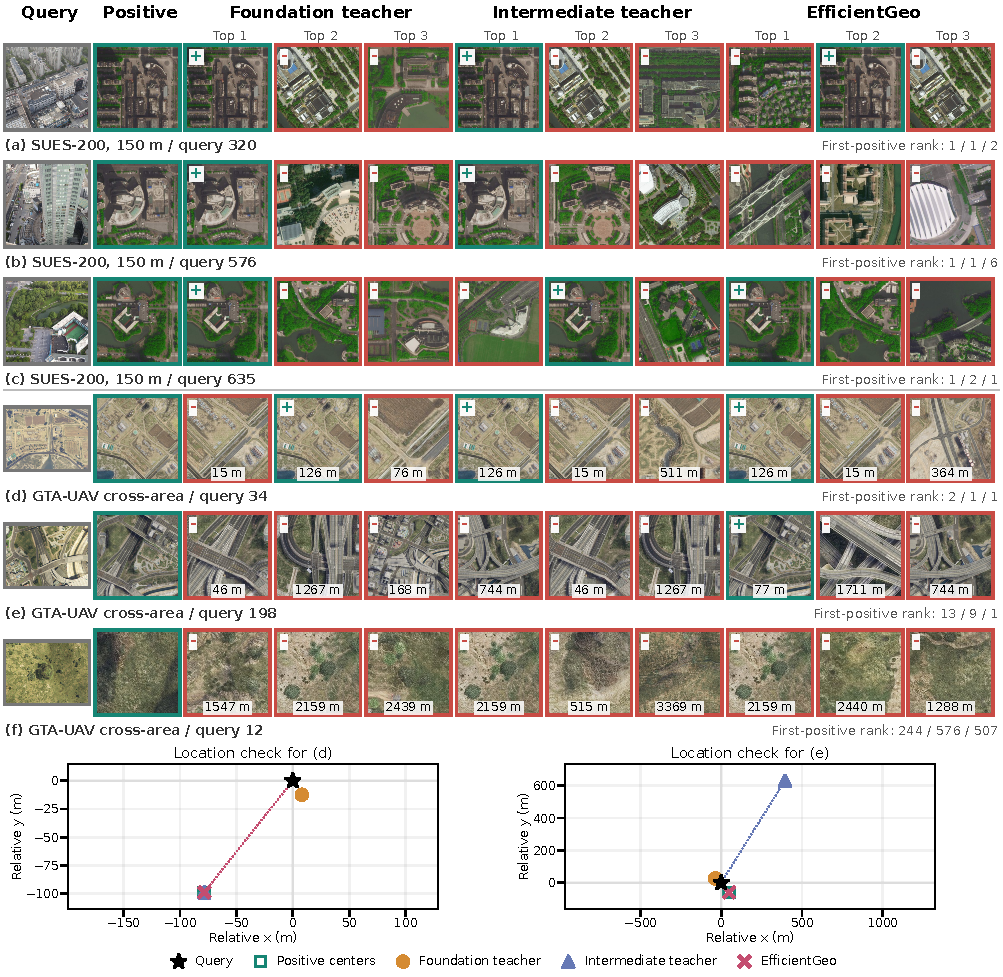
\includegraphics[width=0.88\textwidth]{qualitative_retrieval.pdf}
\caption{Top-3 retrievals on SUES-200 at 150\,m (a--c) and GTA-UAV cross-area (d--f). Green (+) and red ($-$) denote annotated positives and non-positives. First-positive ranks follow the column order: foundation teacher, intermediate teacher, student. The reference is the single SUES-200 positive or the GTA-UAV positive nearest the query. GTA-UAV labels give query-to-tile-center distances; plots show top-1 centers relative to the query. Query IDs are zero-based.}
\label{fig:supp-qualitative}
\endgroup
\end{minipage}\par\addvspace{6pt}
\begin{multicols}{2}
\raggedcolumns
\paragraph{Low-altitude ambiguity and prediction disagreements.}
In (a), the student ranks a similar residential layout above the matching location. In (b), a facade dominates the drone view: both teachers rank the correct location first, but the student ranks it sixth. In (c), the student succeeds where the intermediate teacher ranks the positive second. Across all 150\,m queries, 282 are correct only for the intermediate teacher and 141 only for the student; both succeed on 3,377 and both fail on 200. The cases illustrate layout and facade ambiguities; the counts cover the complete height split.

\paragraph{Exact retrieval versus geographic proximity.}
In (d), the foundation teacher's top-1 is not an annotated positive despite being only 14.8\,m from the query; the other two models retrieve a positive 126.2\,m away. In (e), the student retrieves the correct road junction where both teachers fail. In (f), all three retrieve distant, visually similar vegetation. These cases distinguish exact positive retrieval from geographic proximity.

\end{multicols}

\end{document}



